
\begin{center}
    \emph{\ldots[E]volution codifies happenstance into strategy.\\
    \medskip
    -- \small{from Spillover, by David Quammen.}}
\end{center}
% \newrefcontext[sorting=ynt]

\section*{Abstract}

{
    % \small
    Animal social interactions are the outcomes of evolved strategies that integrate the costs and benefits of being sociable.
    % Using a novel mechanistic, evolutionary, individual-based simulation model, we examine how animals balance the risk of pathogen transmission against the benefits of social information about resource patches, and how this determines the emergent structure of socio-spatial networks.
    We study a scenario in which a fitness-reducing infectious pathogen is introduced into a population which has initially evolved movement strategies in its absence.
    Within only a few generations, pathogen introduction provokes a rapid evolutionary shift in animals' social movement strategies, and the importance of social cues in movement decisions increases.
    Individuals undertake a dynamic social distancing approach, trading more movement (and less intake) for lower infection risk.
    Pathogen-adapted populations disperse more widely over the landscape, and thus have less clustered social networks than their pre-introduction, pathogen-naive ancestors.
    Running epidemiological simulations on these emergent social networks, we show that diseases do indeed spread more slowly through pathogen-adapted animal societies.
    Finally, the mix of post-introduction strategies is strongly influenced by a combination of landscape productivity, the usefulness of social information, and disease cost.
    Our model suggests that the introduction of an infectious pathogen into a population can trigger a rapid eco-evolutionary cascade, rapidly changing animals' social movement strategies, which alters movement decisions and encounters between individuals. 
    In turn, this changes emergent social structures, and our model informs how such change can make populations more resilient to future disease outbreaks.
    Overall, we offer both a modelling framework and initial predictions for the evolutionary and ecological consequences of wildlife pathogen spillover scenarios.

    \bigskip
}

\newpage

\section*{Introduction}

\lettrine{A}{nimal} sociality emerges from individual decisions that balance the benefits of associations against the costs of proximity or interactions with neighbours \autocite[][]{tanner2012,webber2018,webber2022,gil2018}.
While such associations can inadvertently or deliberately yield useful social information about resource availability \autocite{danchin2004,dall2005,gil2018}, they also provide opportunities for the transmission of parasites and infectious pathogens among associating individuals \autocite[][]{weinstein2018,romano2020,albery2021,cantor2021,romano2021}.
Wildlife pathogen outbreaks affect most animal taxa, including mammals \autocite{blehert2009,fereidouni2019,chandler2021,kuchipudi2022}, birds \autocite{wille2022}, amphibians \autocite{scheele2019}, and social insects \autocite{goulson2015}.
Weighing the potential risk of infection from social interactions against the benefits of social movements --- where to move in relation to other individuals' positions --- is thus a common behavioural context shared by many animal species.
Movement strategies incorporating social information --- the presence and status of neighbours --- can facilitate or reduce spatial associations, and help animals balance the costs and benefits of sociality \autocite{albery2021,gil2018,webber2018,webber2022}.
Animals' social movements link landscape spatial structure, individual distributions, and the emergent structure of animal societies \autocite{gil2018,webber2022,kurvers2014}.
Together, they influence the dynamics of disease outbreaks in animal populations \autocite{white2018a,romano2020,romano2021,keeling2001}, and such outbreaks may in turn have cascading effects on landscape structure and community ecology \autocite{monk2022}.

On ecological timescales, pathogen outbreaks often reduce social interactions among individuals.
This is due to a combination of mortality-induced decreases in population density \autocite[e.g.][]{fereidouni2019,monk2022}, and adaptive behavioural responses by which animals reduce encounters between infected and healthy individuals \autocite{stroeymeyt2018,pusceddu2021,stockmaier2021,weinstein2018}.
The latter case includes self-isolating when infected, or avoiding potentially infectious individuals \autocite{stroeymeyt2018,pusceddu2021,stockmaier2021,weinstein2018}.
However, when pathogens are first introduced into a population, such as during novel cross-species spillover \autocite{kuchipudi2022,chandler2021}, fine-tuned avoidance responses are less likely, as individuals may have no prior experience of cues that indicate infection \autocite{weinstein2018,stockmaier2021}.
Spreading through host-host contacts, pathogens causing chronic infections \autocite{bastos2000,jolles2021,vosloo2009} may instead impose fitness costs, thus selecting against host social behaviour, and hence against social connectivity itself \autocite{altizer2003,cantor2021,romano2021,poulin2021,ashby2022}.

% Yet introductions of novel pathogens into wildlife mostly come to light when they result in mass mortality events \autocite{fey2015,wille2022}.
Yet novel pathogen introductions are primarily studied for their immediate demographic \autocite{fey2015}, and potential medical \autocite{wille2022,chandler2021,kuchipudi2022,levi2012} and economic implications \autocite[][]{keeling2001,goulson2015,jolles2021}, with host evolutionary dynamics (and especially changes in sociality) mostly ignored.
This is presumably because the evolution of pathogen host traits, and moreover complex behavioural traits such as sociality, is expected to be slow and not immediately relevant.
Since important aspects of animal ecology, including the transmission of foraging tactics \autocite{klump2021} and migration routes \autocite{jesmer2018,guttal2010}, depend on social interactions, it is necessary to understand the long-term consequences of pathogen introductions for animal societies.
Climate change is only expected to make novel pathogen introductions more common \autocite{sanderson2020,carlson2022a}, making such studies more urgent.

Theory suggests that animal sociality evolves to balance the value of social associations against the risk of pathogen transmission \autocite[][]{bonds2005,prado2009,ashby2022}.
However, analytical models often reduce animal sociality to single parameters, while it actually emerges from individual decisions conditioned on multiple internal and external cues.
Social decision-making and movement often also vary among individuals \autocite{tanner2012,wolf2012,spiegel2017,gartland2021}, but analytical models are unable to include individual differences in sociability.
Epidemiological models based on contact networks can incorporate individual variation in social behaviour by linking these differences to positions in a social network \autocite{white2017,albery2021,albery2020}.
Yet network models often cannot capture fine-scale feedbacks between individuals' social and spatial positions \autocite{albery2021,albery2020}, nor spatial variation in infection risk \autocite{albery2022}, making such models sensitive to both the network formation process, and to sampling biases in empirical data collection \autocite[][]{white2017}.

Mechanistic, individual-based simulation models (IBMs) suggest themselves as a natural solution; they can incorporate substantial ecological detail, including explicit spatial settings \autocite{deangelis2019}, and detailed disease transmission \autocite{white2018, scherer2020,lunn2021,white2018a}.
Individual-based models hitherto haved focused on immediate epidemiological outcomes, such as infection persistence, and do not have an evolutionary component \autocite{white2018,scherer2020,lunn2021}.
Incorporating an evolutionary component to movement-disease IBMs could allow predictions on important feedbacks between the ecological outcomes of infectious disease and the consequences for the evolution of host behaviour \autocite{cantor2021}.
This could include the emergence of tradeoffs in the costs and benefits of sociability \autocite{gartland2021}, with cascading ecological and social effects \autocite{monk2022,spiegel2017,tanner2012,webber2022}.
The range of animal taxa at risk from a wide array of pathogens and parasites \autocite{carlson2022a,sanderson2020} makes it important to conceive of models that can capture the key features of diverse host-pathogen dynamics and offer broad conceptual insights \autocite{white2018a,white2018}.

We built a model that seeks to capture the essential elements of pathogen (or parasite) transmission among animals foraging on patchily distributed resources --- this is a common behavioural context shared by many potential host species \autocite{white2018a,white2018}.
We examined the eco-evolutionary consequences of the introduction of a pathogen into a novel host population \autocite[such as during cross-species spillover:][]{blehert2009,bastos2000,wille2022,fereidouni2019,scheele2019,sanderson2020,carlson2022a,kuchipudi2022,monk2022}.
In our evolutionary, spatial, individual-based simulation, we modelled the repeated introduction of an infectious pathogen to populations that had already evolved foraging movement strategies in its absence.
Our model could be conceived as an abstract representation of, among others, spillovers of foot-and-mouth disease from buffalo to impala \autocite{bastos2000,vosloo2009}, or sarcoptic mange from llamas to vicu\~nas \autocite{monk2022}, current and historic spread of avian influenza among sea- and wading bird species \autocite{globconsorth5n82016,wille2022}, or SARS-CoV-2 from humans to deer \autocite{chandler2021,kuchipudi2022}.

We compared how social information was used in movement strategies evolved before and after pathogen introduction, and the ecological outcomes for individual intake, movement, and associations with other foragers.
Using both IBMs and network epidemiological models \autocite{wilber2022,stroeymeyt2018,white2017,bailey1975}, we examined whether pathogen-risk adapted populations were more resilient to the spread of infectious disease than their pathogen-risk naive ancestors.
We also investigated the effect of landscape productivity and the cost of infection, which are both expected to influence the selection imposed by pathogen transmission \autocite{ezenwa2016,almberg2015,hutchings2000}.
Overall, we provide a theoretical framework broadly applicable to novel host-pathogen introduction scenarios, and demonstrate the importance of including evolutionary dynamics in movement-disease models.

\section*{The Pathomove Model of Novel Pathogen Introduction}

We implemented an individual-based simulation model to represent foraging animals (`foragers') seeking discrete, immobile, depleteable food items (see \textit{SI Appendix Fig. S1 -- S2}) \autocite{spiegel2017,gupte2021a}.
Food items are distributed over a two-dimensional, continuous-space resource landscape with wrapped boundaries (a torus).
Our model, similar to previous eco-evolutionary individual based models \autocite{getz2015, netz2021, gupte2021a}, has two distinct timescales: (1) an ecological timescale comprising of \textit{T} timesteps that make up one generation ($T$ = 100 by default), and (2) an evolutionary timescale consisting of 5,000 generations (G).
At the ecological timescale, individuals sense local counts of food items and competitors, move according to inherited movement strategies, and forage for food.
At the same timescale, individuals that carry an infectious, fitness-reducing pathogen, may, when in close proximity with uninfected individuals, pass on the pathogen with a small probability (see \textit{Pathogen Transmission and Disease Cost}).
At the evolutionary timescale, individuals reproduce and transmit their movement strategies (see \textit{Starting Location and Inheritance of Movement Rules}) to the their offspring. The number of offspring is linked both to individuals' success in finding and consuming food items, and to the duration that they were infected by the pathogen at the ecological timescale.
The model was implemented in R and C++ using Rcpp \autocite{rcoreteam2020,eddelbuettel2013} and the \textit{Boost.Geometry} library for spatial computations (\textit{www.boost.org}); model code is at \textit{github.com/pratikunterwegs/pathomove}.

\subsection*{Distribution of Food Items}

Our landscape of 60 $\times$ 60 units contains 1,800 discrete food items, which are clustered around 60 resource `kernels', for a resource density of 0.5 items per unit\textsuperscript{2} (see \textit{SI Appendix Fig. S1 -- S2}).
% Food items are initialised to become available after some $t$ timesteps, where $t$ is drawn from a Poisson distribution with a mean of 10 (10\% of the regeneration time; see below).
This prevents synchronicity in the availability and regeneration of food items.
Each available food item can be sensed and harvested by foraging individuals (see below).
Once harvested, another food item is regenerated at the same location after a fixed regeneration time R, which is set at 50 timesteps by default; alternative values of 20 and 100 timesteps represent high and low productivity landscapes respectively.
Food item regeneration is delinked from population generations.
Thus the actual number of available food items is almost always in flux.
In our figures and hereafter, we chose to represent R as the number of times a food item would regenerate within the timesteps in a single generation $T$ (default = 100), resulting in R values of 1, 2, and 5 for regeneration times of 100, 50 (the default), and 20 timesteps.
Items that are not harvested remain on the landscape until they are picked up by a forager.
Each food item must be processed, or `handled', by a forager for $T_H$ timesteps (the handling time, default = 5 timesteps) before it can be consumed \autocite{ruxton1992,gupte2021a}.
The handling time dynamic is well known from natural systems in which there is a lag between finding and consuming a food item \autocite{ruxton1992}, and may be caused by the need to extract edible portions from inedible structures, such as mussels from their shells, or seeds from their casings.

\subsection*{Individual Foraging and Movement}

Individuals forage in a randomised order, harvesting the first available food item within their movement and sensory range ($d_S$ = $d_M$, a circle with a radius of 1 unit (see \textit{SI Appendix Fig. S1 -- S2}).
Once harvested, the item is no longer available to other individuals, leading to exploitation competition among nearby foragers.
Furthermore, the location of the item also yields no more cues to other foragers that an item will reappear there, reducing direct cues by which foragers can navigate to profitable clusters of food items.
Individuals that harvest a food item must handle it for $T_H$ timesteps (default = 5 timesteps), while all individuals not handling a food item are considered idle \autocite{ruxton1992,gupte2021a}.
As handlers are immobilised at the location where they encountered food, they may be good indirect indicators of the location of a resource cluster (`social information') \autocite[][]{danchin2004,romano2020,gupte2021a}.
Once individuals finish handling a food item, they return to the non-handling, searching state.

Our model individuals move in small, discrete steps of fixed size ($d_M$ = 1 unit).
Each step is chosen based on the individuals' assessment of local environmental cues, and this assessment is made using evolved movement strategies \autocite[as in][]{netz2021,gupte2021a}.
First, individuals scan their current location, and five equally spaced points around their position, at a distance of 1 unit for three cues ($d_S$, see \textit{SI Appendix Fig. S1 -- S2}): the number of food items ($F$), the number of foragers handling a food item (`handlers': $H$) and the number of idle foragers not handling a food item (`non-handlers': $N$).
Individuals assign a suitability \autocite[see][]{netz2021,gupte2021a} to their current position and each of the five locations, using their inherited preferences for each of the cues: $S = s_FF + s_HH + s_NN$ + $\epsilon$.
The preferences $s_F$, $s_F$, and $s_N$ for each of the three cues are heritable from parents to offspring, while $\epsilon$ is a very small error term drawn for each location, to break ties among locations.
The values of each of the cue preferences \emph{relative to each other} determine individuals' movement strategies \autocite{gupte2021a}.
All individuals move simultaneously to the location to which they have assigned the highest suitability (`step selection') \autocite[akin to step-selection;][]{fortin2005}; this may be their current location, in which case individuals are stationary for that timestep.
Since individuals may differ in their inherited preferences for each of the three cues, two individuals at the same location may make quite different movement decisions based on the same local cues.
Handlers, however, are considered immobile and do not make any movement decisions.

\subsection*{Pathogen Transmission and Disease Cost}

We modelled circumstances that are expected to become increasingly common due to rapid global changes; the population evolves for $3/5$\textsuperscript{th} of the simulation (until G = 3,000; of 5,000) in the absence of a pathogen, after which a pathogen is introduced in each generation until the end of the simulation (G = 5,000).
Our model captures some essential features of pathogen or parasite transmission among animals \autocite{white2017}: the pathogen may transmit from infected host individuals to their susceptible neighbours with a per-timestep probability $p$ of 0.05.
This transmission is only possible when the two individuals are within a the transmission distance, $d_\beta$.
For simplicity, we set $d_\beta$ to be the movement range (1 unit).
Once transmitted, the pathogen is assumed to cause a chronic disease which reduces host energy stores by a fixed amount called $\delta E$ in every following timestep; $\delta E$ is set to 0.25 by default (alternative values: 0.1, 0.5).
Since novel pathogen introductions can periodically re-occur in natural environments \autocite{jolles2021,bastos2000,vosloo2009,almberg2015,goulson2015,wille2022,carlson2022a}, we set up our model such that the pathogen was introduced to 4\% of individuals in each generation (N = 20; `primary infections').
This is necessary to kick-start the pathogen-movement eco-evolutionary feedback dynamics, and populations may indeed repeatedly acquire novel pathogens (or strains) through external sources, such as infected individuals of other spatially overlapping species \autocite[e.g.][]{kuchipudi2022,wille2022,chandler2021,vosloo2009,bastos2000,monk2022,keeling2001,carlson2022a}.
For completeness, we also considered scenarios in which novel pathogen introductions only occur sporadically in the generations after the initial event, rather than in every generation (see \emph{SI Appendix}).

\subsection*{Starting Location and Inheritance of Movement Rules}

For simplicity, we considered a population of haploid individuals with discrete, non-overlapping generations, and asexual inheritance.
At the end of the parental generation, the net lifetime energy of each individual was determined as the difference of the total energy gained through food intake and the energy lost through infection. 
In the \textit{SI Appendix}, we also consider an alternative implementation in which potential immune resistance against the pathogen requires a certain percentage of individual intake, reducing the value of each food item.
The parental population produces an offspring population (of the same size) as follows: to each offspring, a parent is assigned at random by a weighted lottery, with weights proportional to lifetime net energy (an algorithm following the replicator equation) \autocite{hofbauer1988,hamblin2013}.
This way, the expected number of offspring produced by a parent is proportional to the parent's lifetime success \autocite{hofbauer1988}.
The movement decision-making cue preferences $s_F$, $s_H$, and $s_N$ are subject to independent random mutations with a probability of 0.01.
The mutational step size (either positive or negative) is drawn from a Cauchy distribution with a scale of 0.01 centred on zero.
Thus, while the majority of mutations are small, there can be a small number of very large mutations.
As in real ecological systems, individuals in the new generation are intialised around the location of their parent (within a standard deviation of 2.0), and thus successful parents give rise to local clusters of offspring (see an alternative implementation in \textit{SI Appendix}).

\subsection*{Model Output}

To understand the evolution of movement strategies, and especially how individuals weighed social information, we recorded the population's evolved cue preferences in every second generation, and interpreted them using the `behavioural hypervolume' approach \autocite{bastille-rousseau2019}.
We classified individuals based on how they used social information --- the presence and status of competing foragers --- into four social movement classes: (1) agent avoiding, if $s_H, s_N < 0$, (2) agent tracking, if both $s_H, s_N > 0$, (3) handler tracking, if $s_H > 0, s_N < 0$, and (4) non-handler tracking, if $s_H < 0, s_N > 0$.
We calculated the relative importance of social cues --- $H, N$ --- to each individual's movement strategy as $ SI_{imp} = (|s_H| + |s_N|) / (|s_H| + |s_N| + |s_F|)$, with higher values indicating a greater importance of social cues.

Animal movements and foraging distributions provide opportunities for between-individual associations, which usually have a spatial context.
Associations which depend on spatial proximity can be captured at the individual- and population-level by proximity-based animal social networks \citep{whitehead2008,farine2015}.
Social networks measured from empirical studies have been broadly informative about the structure of animal societies, and the consequences of this structure for animal culture, such as the learning of migration routes or foraging skills \citep{aplin2012,aplin2013,cantor2021}, and for disease transmission \citep{stroeymeyt2018,albery2021,cantor2021}.
%%
We created a proximity-based adjacency matrix by counting the number of times each individual was within the sensory and pathogen transmission distance $d_\beta$ (= $d_S, d_M$ = 1 unit) of another individual \citep{whitehead2008,wilber2022}.
We transformed this matrix into an undirected social network weighted by the number of pairwise encounters: in a pairwise encounter, both individuals were considered to have associated with each other \citep{white2017}.
The strength of the connection between any pair was the number of times the pair were within $d_\beta$ of each other over their lifetime.
%%
We logged encounters and constructed social networks after every 10\% of the total generations (i.e., every 500\textsuperscript{th} generation), and at the end of the simulation.
We constructed adjacency matrices using Rcpp \citep[][]{eddelbuettel2013}, and converted them to networks using the \textit{igraph} \citep{csardi2006} and \textit{tidygraph} \citep{pedersen2020} libraries for R.
We omitted ephemeral pairwise associations with a weight $<$ 5.

We plotted the mix of social information-based movement strategies evolved across generations in each parameter combination.
Focusing on our default scenario ($\delta E$ = 0.25, R = 2), we visualised the mean per-capita distance moved, mean per-capita intake, and mean per-capita encounters with other foragers.
We examined how the three main social movement strategies --- agent avoidance, agent tracking, and handler tracking --- changed in frequency over generations.
We also examined differences among strategies in the movement distance, associations with other agents, and frequency of infection, after they had reached an eco-evolutionary equilibrium following pathogen introduction (G > 3,500).
We visualised the proximity based social networks of populations in a representative scenario ($\delta E$ = 0.25, R = 2), focusing on the generations just before and after the pathogen introduction events begin (pre-introduction: G = 3,000; post-introduction: G = 3,500).
We plotted the numbers of individuals infected in each generation after pathogen introduction to examine whether evolutionary changes in movement strategies actually reduced infection spread.
We also ran simple network epidemiological models on the emergent individual networks in generations 3,000 and 3,500 \autocite{bailey1975,white2017,stroeymeyt2018,wilber2022}, for robust comparisons of potential pathogen spread in pathogen-naive and pathogen-adapted populations, respectively.

\section*{Outcomes from the Pathomove Model}

In our model, individuals move and forage on a landscape with patchily distributed food items, and select where next to move in their vicinity, based on inherited preferences for environmental cues --- food items, and other individuals (see \textit{SI Appendix Fig. S1}).
Food items, once consumed, regenerate at a rate R, and pathogen infection imposes a per-timestep cost $\delta E$.
We classified individuals' social movement strategies in our model using a simplified `behavioural hypervolume' approach \autocite{bastille-rousseau2019}, based on the sign of their preferences for successful foragers handling a food item (`handlers', preference $s_H$), and for unsuccessful foragers still searching for food (`non-handlers', preference $s_N$).
In our default scenario, R = 2, food regenerates twice per generation, and $\delta E$ = 0.25, i.e., consuming 1 food item offsets 4 timesteps of infection. 
Over the 3,000 generations before the introduction of the pathogen, populations reached an eco-evolutionary equilibrium where the commonest social movement strategy was to prefer moving towards both handlers and non-handlers (`agent tracking'; $s_H, s_N > 0$; but see below) (Fig.~\ref{fig_eco_evo_general}A).

\subsection*{Rapid Evolutionary Shift in Social Movement Strategies Following Pathogen Introduction}

Introducing an infectious pathogen to 4\% (n = 20) of individuals in each generation (after G = 3,000), leads to a remarkably rapid evolutionary shift --- within only 25 generations of pathogen introduction --- in how social information is incorporated into individuals' movement strategies.
There is a marked increase in the frequency of individuals that track successful foragers, but avoid non-handlers (`handler tracking'; $s_H > 0$, but $s_N < 0$) (Fig.~\ref{fig_eco_evo_general}A; 3,000 $< G <$ 3,025).
Surprisingly, after a brief period (in evolutionary terms) of handler tracking being the most common strategy, a third strategy also becomes more common: avoiding both handlers and non-handlers (`agent avoiding'; $s_H, s_N < 0$).
Within 250 generations after pathogen introduction, agent avoiding becomes as common as the handler tracking strategy, and this appears to be a stable equilibrium that is maintained until the end of the simulation (2,000 generations after pathogen introduction; Fig.~\ref{fig_eco_evo_general}A).
The \textit{SI Appendix} shows how the occurrence of rapid evolutionary shifts is broadly robust to modelling assumptions; in brief, such shifts occur even when individuals cannot benefit from evolved adaptation to local conditions \autocite{badyaev2009}, and when the pathogen saps a percentage, rather than an absolute value, from daily intake.

In addition to qualitative changes in social movement strategies, pathogen introduction also leads to social information becoming more important to movement decisions.
Prior to pathogen introduction ($G <$ 3,000), individuals' handler- and non-handler preferences ($|s_H| + |s_N|$; taken together, social information) barely influence their movement strategies (Fig.~\ref{fig_eco_evo_general}B).
These are instead guided primarily by the preference for food items ($s_F$; see \textit{Model and Analysis}; see also \textit{Supplementary Information}).
Social movement decisions are joint outcomes of individual preferences for social cues and the cue value: consequently, in clustered populations (see below), even small positive values of $s_H$ and $s_N$ lead to strong emergent sociality.
After pathogen introduction, there is a substantial increase in the average importance of individuals' preferences (or aversions) for the presence of other foragers (Fig.~\ref{fig_eco_evo_general}B).
However, there is significant variation among individuals in the importance of social information to their movement strategies, with distinct evolved polymorphisms that vary substantially between simulation replicates (Fig.~\ref{fig_eco_evo_general}B).

\begin{figure}[!h]
    \centering
    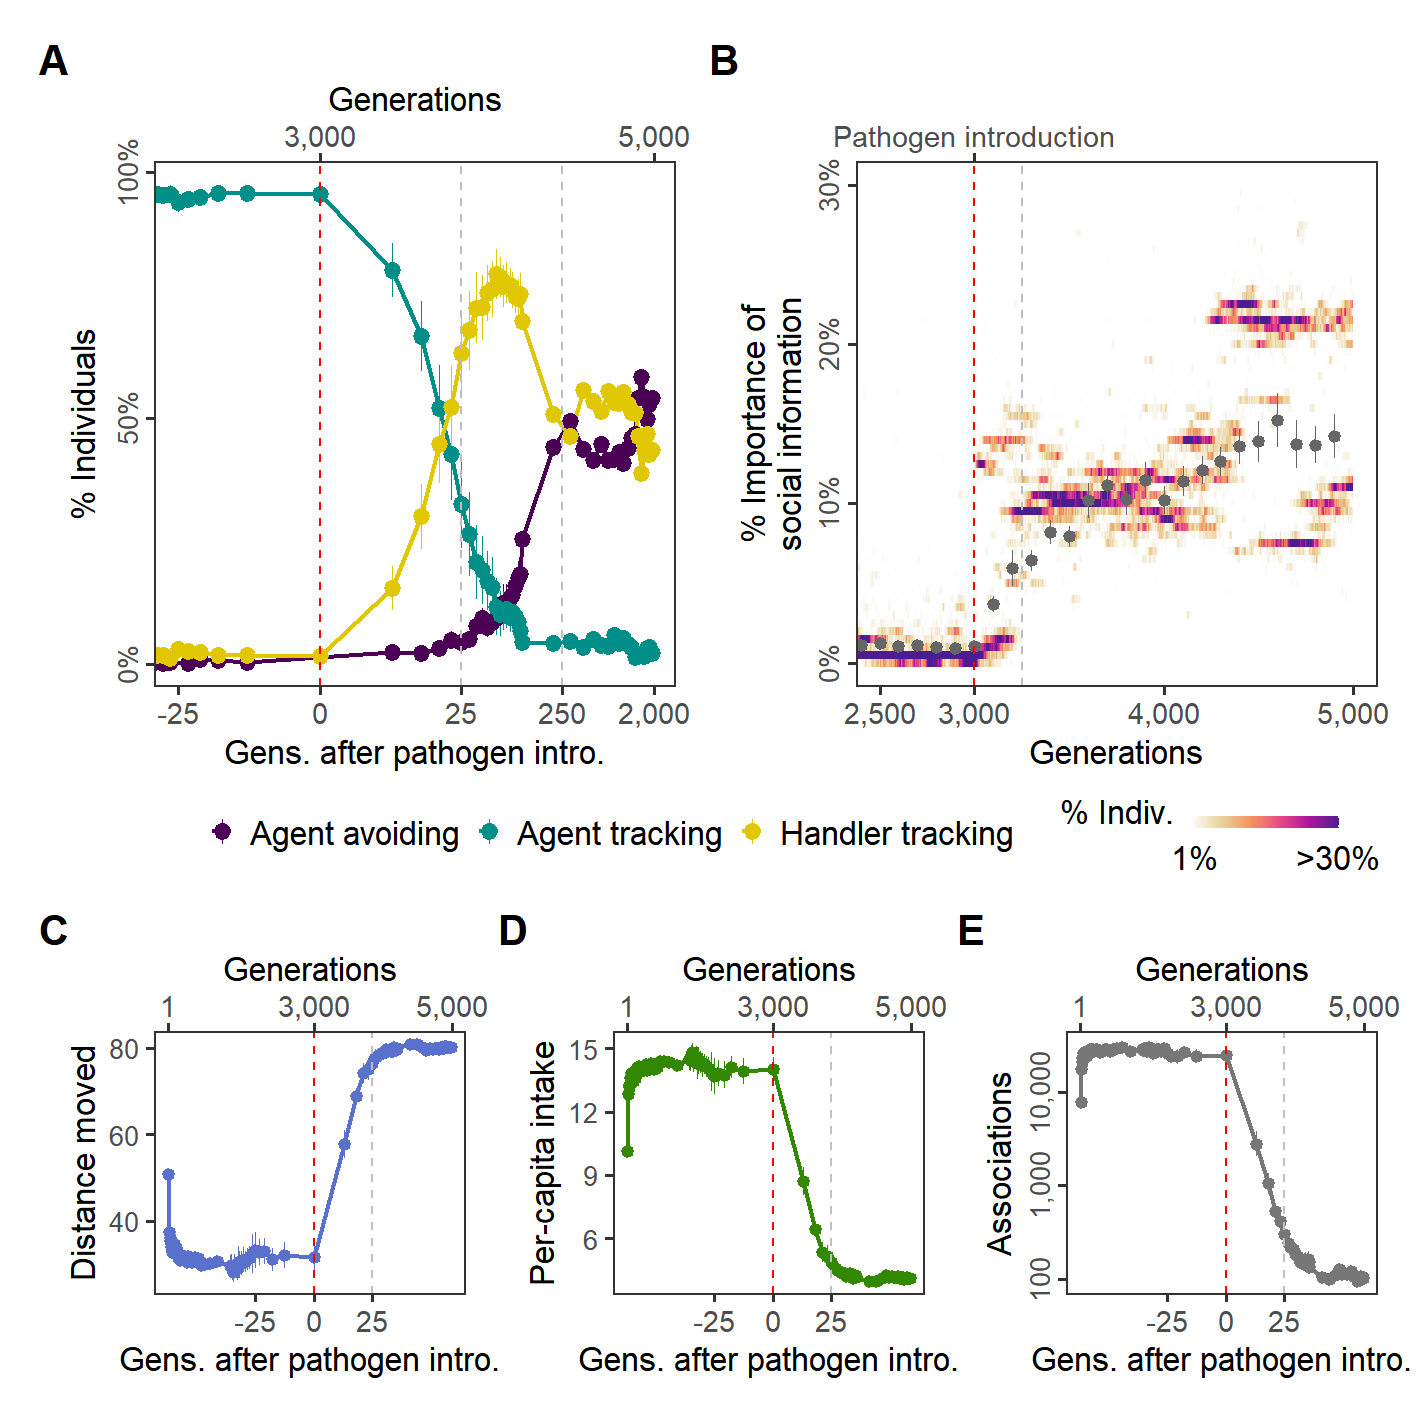
\includegraphics[width=0.8\linewidth]{figures/pathomove/fig_eco_evo_general.png}
    \caption{
        \textbf{Pathogen introduction leads to rapid evolutionary changes in social information use, with cascading effects on population ecological outcomes.}
        \textbf{(A)} Before pathogen introduction in the default scenario (R = 2, $\delta E$ = 0.25), populations rapidly evolve a social movement strategy that tracks all other individuals (`agent tracking'; $G \leq$ 3,000) --- however, their overall movement strategy is primarily guided by the presence of food items \textbf{(B)}.
        Pathogen introduction leads to the rapid replacement, within 25 generations, of agent tracking with `handler tracking' (preference for successful foragers; 3,000 $< G <$ 3,025). 
        Within 250 generations, `agent avoidance' (avoidance of both successful and unsuccessful foragers; $G >$ 3,250) also becomes common, stably co-existing with the handler tracking strategy in an eco-evolutionary equilibrium.
        \textbf{(B)} After pathogen introduction ($G >$ 3,000), the importance of social cues (the presence of other individuals; the sum of the absolute, normalised preferences $sH, sN$) increases substantially on average (grey points).
        Additionally, there is significant variation in the importance of social cues to individuals (shaded regions), which is not captured by the mean or standard error.
        At G = 4,500, for example, social information comprises $\approx$ 10\% of some individuals' movement strategies, but some individuals have evolved a stronger weight for social cues ($>$ 20\%).
        The rapid change in social movement strategies following pathogen introduction has cascading effects on ecological outcomes.
        Individuals, which have evolved strong aversions to at least some kinds of foragers (depending on their strategy), \textbf{(C)} move more on average, \textbf{(D)} have only 25\% of the pre-pathogen average intake, and \textbf{(E)} have 100-fold fewer associations with other individuals.
        All panels show data averaged over 10 replicates, but shaded region in panel B shows only a single replicate for clarity.
    }
    \label{fig_eco_evo_general}
\end{figure}

\subsection*{Disease-dominated Ecological Cascade Due to Evolutionary Shift in Movement Strategies}

The evolutionary shift in social movement strategies causes a drastic change in ecological outcomes (Fig.~\ref{fig_eco_evo_general}C -- E; see \textit{SI Appendix Fig. S3} for other scenarios).
There is a sharp increase in mean distance moved by individuals; while pre-introduction individuals moved 35\% of their lifetimes on average (i.e., 35 timesteps; handling for the remainder), post-introduction, individuals move for 80\% of their lifetimes (i.e., 80 timesteps; Fig.~\ref{fig_eco_evo_general}C).
The handler tracking and agent avoiding strategies lead individuals to move away from groups of individuals \autocite[`dynamic social distancing';][]{pusceddu2021}.
Individuals being most likely to be found near resource clusters, this leads to movement away from productive areas of the landscape.
Consequently, there is a rapid, four-fold drop in mean per-capita intake after pathogen introduction (Fig.~\ref{fig_eco_evo_general}D).
The concurrent, near 100-fold drop in encounters between individuals after pathogen introduction (Fig.~\ref{fig_eco_evo_general}E) suggests that most encounters were likely taking place on or near resource clusters.
The reductions in intake observed are equivalent to those expected from halving landscape productivity (\textit{SI Appendix Fig. S3}).
Our model shows how even a non-fatal pathogen, by influencing the evolution of movement strategies, can have substantial indirect ecological effects --- a disease dominated ecological cascade \autocite{monk2022}.

\subsection*{Co-existence of Social Movement Strategies}

At eco-evolutionary equilibrium (G $>$ 3,500) the relationship between movement and avoiding associations (and further, infection) is mediated by individual differences in how exactly social information is incorporated into movement strategies.
Individuals using the agent avoiding strategy move more than handler tracking ones (Fig.~\ref{fig_social_outcomes}A), about 85\% of their lifetime (default scenario: R = 2; $\delta E$ = 0.25).
At this limit, every step moved allows them to avoid approximately 2 encounters with other individuals.
Handler tracking individuals move much less ($\sim$ 60\% -- 80\%), but are able to avoid approximately 20 encounters with other individuals with every extra step.
These differences may explain why agent avoiding and handler tracking individuals have similar mean infection rates, at $\sim$ 25\% and $\sim$ 33\% respectively (Fig.~\ref{fig_social_outcomes}B).
All other strategies, especially the agent tracking strategy common in pre-introduction populations, are barely able to translate increased movement into fewer associations (Fig.~\ref{fig_social_outcomes}A).
These strategies have a wide range of infection rates (Fig.~\ref{fig_social_outcomes}B), potentially because they are very rare --- these likely represent mutants that do not give rise to persistent lineages.

\begin{figure}[!h]
    \centering
    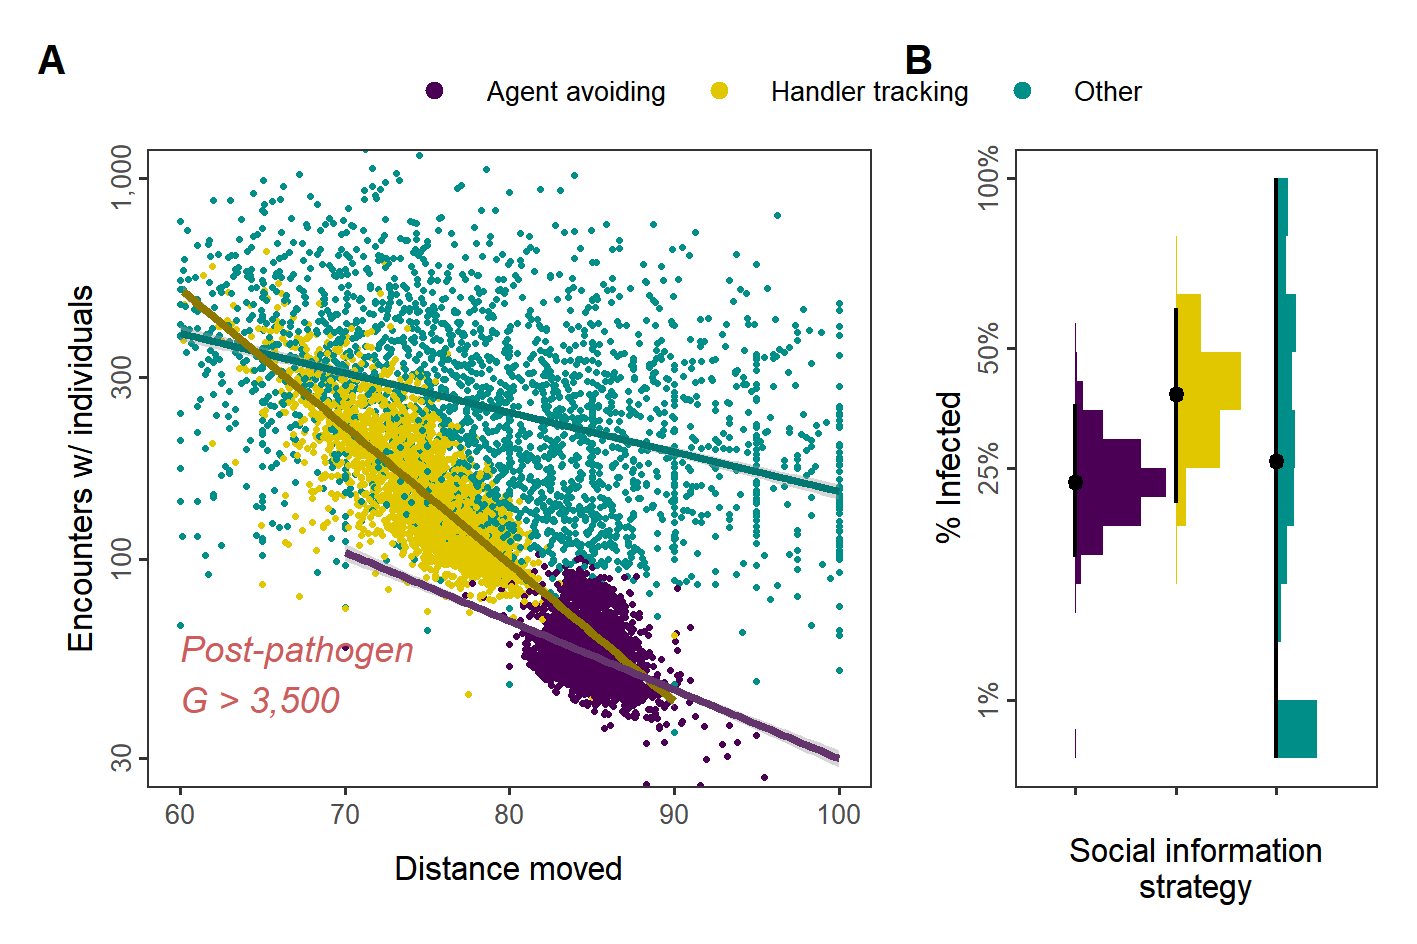
\includegraphics[width=0.8\linewidth]{figures/pathomove/fig_social_outcomes.png}
    \caption{
        \textbf{Social movement strategies trade movement for associations through dynamic social distancing, leading to differences in infection rates.}
        In post-introduction populations at eco-evolutionary equilibrium (G $>$ 3,500), \textbf{(A)} both agent avoiding and handler tracking individuals can reduce encounters with other individuals by moving to avoid other foragers (dynamic social distancing).
        Handler tracking individuals have many more encounters than agent avoiding individuals, but surprisingly, are better able to reduce encounters through increased movement.
        Individuals using other strategies (mostly agent tracking) have a wider range of movement distances, but cannot efficiently avoid other foragers by moving more.
        \textbf{(B)} Avoiding all other foragers leads to marginally lower infection rates than tracking successful foragers (and avoiding unsuccessful ones; handler tracking).
        Surprisingly, rare pre-introduction strategies such as following any nearby individuals (agent tracking) may also have low infection rates, potentially due to their rarity.
        Panel A shows linear model fits with a log scale Y-axis; panel B shows infection rates; all data represent generation- and replicate-specific means (G $>$ 3,500; R = 2, $\delta E$ = 0.25).
    }\label{fig_social_outcomes}
\end{figure}

\subsection*{Reorganisation of Spatial-social Structure}

Following pathogen introduction, the mixture of individual-level movement strategies elicits a substantial re-organisation of emergent spatial and social structure at the population level.
Pre-introduction populations are strongly clustered in space (Fig.~\ref{fig_networks_disease}A), due to movement strategies that favour following most other foragers.
This spatial proximity means that most individuals encounter each other at least once, leading to numerous unique partners (the `degree') for each forager (Fig.~\ref{fig_networks_disease} inset 1: \emph{blue}).
In contrast, the spread-out networks in pathogen-risk adapted populations suggest that most foragers move substantially from their initial locations over their lifetime, associating only ephemerally with foragers from all over the landscape (Fig.~\ref{fig_networks_disease}B).
This reflects movement strategies which lead to near-perpetual movement to avoid associations; a sort of dynamic social distancing seen in real animal societies under risk of pathogen spread \autocite{weinstein2018,stroeymeyt2018,pusceddu2021,stockmaier2021}.
This dispersed population structure means that most pathogen-risk adapted foragers encounter fewer than 10\% of the population over their lifetime (Fig.~\ref{fig_networks_disease} inset 1: \emph{red}).

\afterpage{
\begin{figure*}[!h]
    \centering
    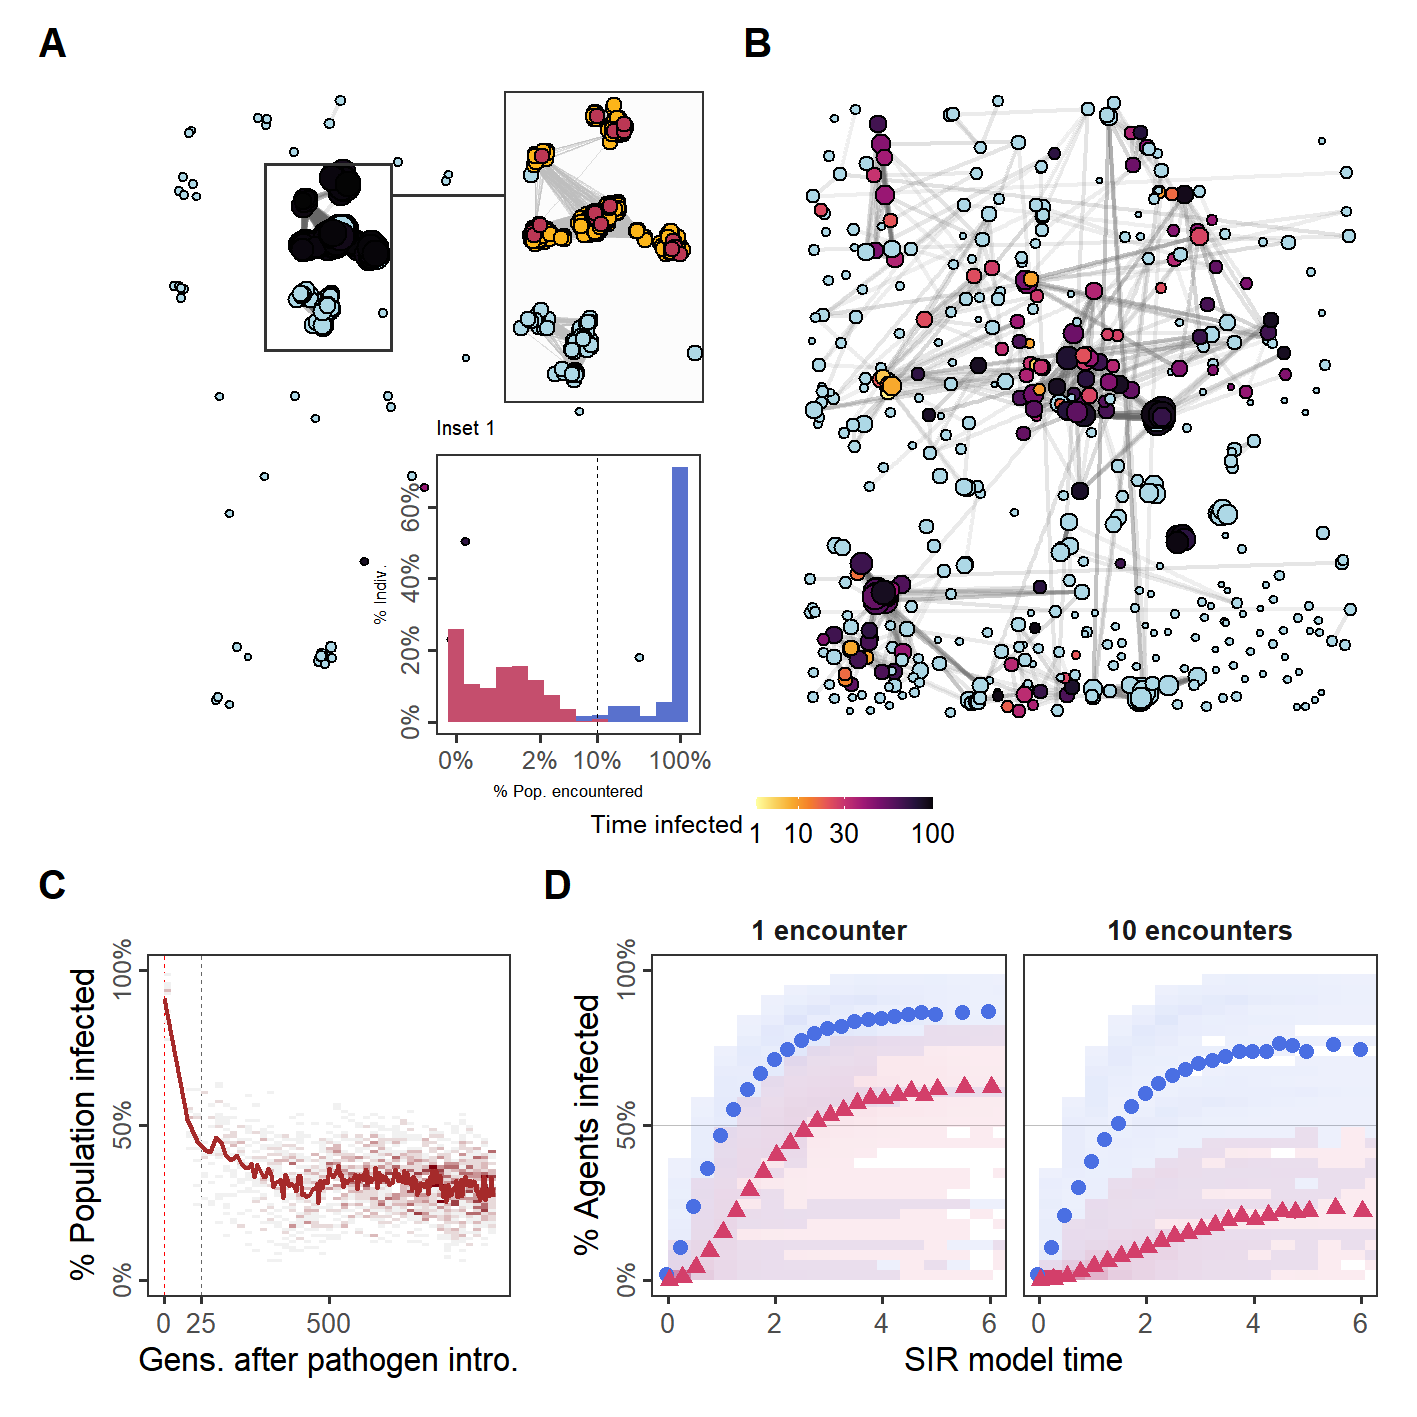
\includegraphics[width=0.8\linewidth]{figures/pathomove/fig_networks_disease.png}
    % width=8.7cm
    \caption{
        \textbf{Reduced spatial-social clustering and disease transmission in populations adapted to the presence of an infectious pathogen.}
        pathogen-risk naive populations (\textbf{A}; G = 3,000) are much more spatially clustered than pathogen-risk adapted populations (\textbf{B}; G = 3,500), and are thus rapidly infected (red: primary infections; yellow: secondary infections; blue: never infected).
        Pre-introduction individuals encounter many more unique neighbours (\textbf{inset 1}, blue) than pathogen-risk adapted individuals (\textbf{inset 1}; red). 
        Dashed grey line represents 10\% of individuals encountered (N = 50).
        Main panels show social networks from a single replicate of the default scenario (R = 2, $\delta E$ = 0.25), insets show 10 replicates. Nodes represent individuals positioned at their final location. Connections represent pairwise encounters, and node size represents encounters (larger = more encounters). Darker node colours indicate longer infection (light blue = no infection). 
        \textbf{(C)} In the first generations following pathogen introduction, nearly every single individual in the population is infected. However, within 25 generations, tracking the evolutionary shift towards movement strategies that avoid some or all other individuals, only about 50\% of individuals are ever infected; this drops to a stable 30\% within 500 generations after pathogen introduction.
        \textbf{(D)} The progression of two hypothetical diseases, requiring a single encounter, or 10 encounters for a potential transmission, on emergent social networks. 
        The transmission of both diseases is reduced in populations with disease-adapted movement strategies (pre-introduction: G = 3,000, blue circles; post-introduction: G = 3,500, red triangles). Subfigures in panel D show means of 25 SIR model replicates (transmission rate $\beta$ = 5.0, recovery rate $\gamma$ = 1.0), run on emergent social network; both panels represent 10 simulation replicates the default scenario.
    }\label{fig_networks_disease}
\end{figure*}
}

\subsection*{Pathogen-risk Adapted Movement Strategies Make Animal Societies More Resilient to the Spread of Disease}

Nearly every individual in the generations just after pathogen introduction was infected.
However, tracking the evolutionary change in movement strategies, the number of infected individuals fell to just about 50\% within 25 generations (Fig.~\ref{fig_networks_disease}C).
To examine potential pathogen spread in pre-introduction populations, we ran a simple epidemiological model on the social networks emerging from individuals' movements before and after pathogen introduction (pre-introduction: G = 3,000; post-introduction: G = 3,500).
We modelled two diseases, \textit{(i)} first, a disease requiring one encounter,and \textit{(ii)} second, a disease requiring ten encounters between individuals for a potential transmission event (transmission rate $\beta$ = 5.0, recovery rate $\gamma$ = 1.0).

Both the single encounter and multiple encounter diseases would infect 75\% -- 80\% of individuals when spreading through the networks of pre-introduction populations (Fig.~\ref{fig_networks_disease}D).
Pathogen-risk adapted populations' social networks are more resilient to both the single encounter and multiple encounter disease, compared to their pre-introduction, pathogen-risk naive ancestors, as these social networks are sparser and individuals are more weakly connected (Fig.~\ref{fig_networks_disease}D).
Less than 60\% of post-introduction populations were finally infected by the single encounter disease, compared with $>$ 75\% of pre-introduction, pathogen-risk naive ancestors; in pathogen-risk adapted populations, the spread of the multiple encounter disease was even slower (ever infected: $\approx$ 20\%).
% the infection peak in pathogen-adapted networks  was only about half as much as for their pathogen-naive ancestors' networks (25\% \textit{versus} 50\% of individuals).

\afterpage{
\begin{figure}[!h]
    \centering
    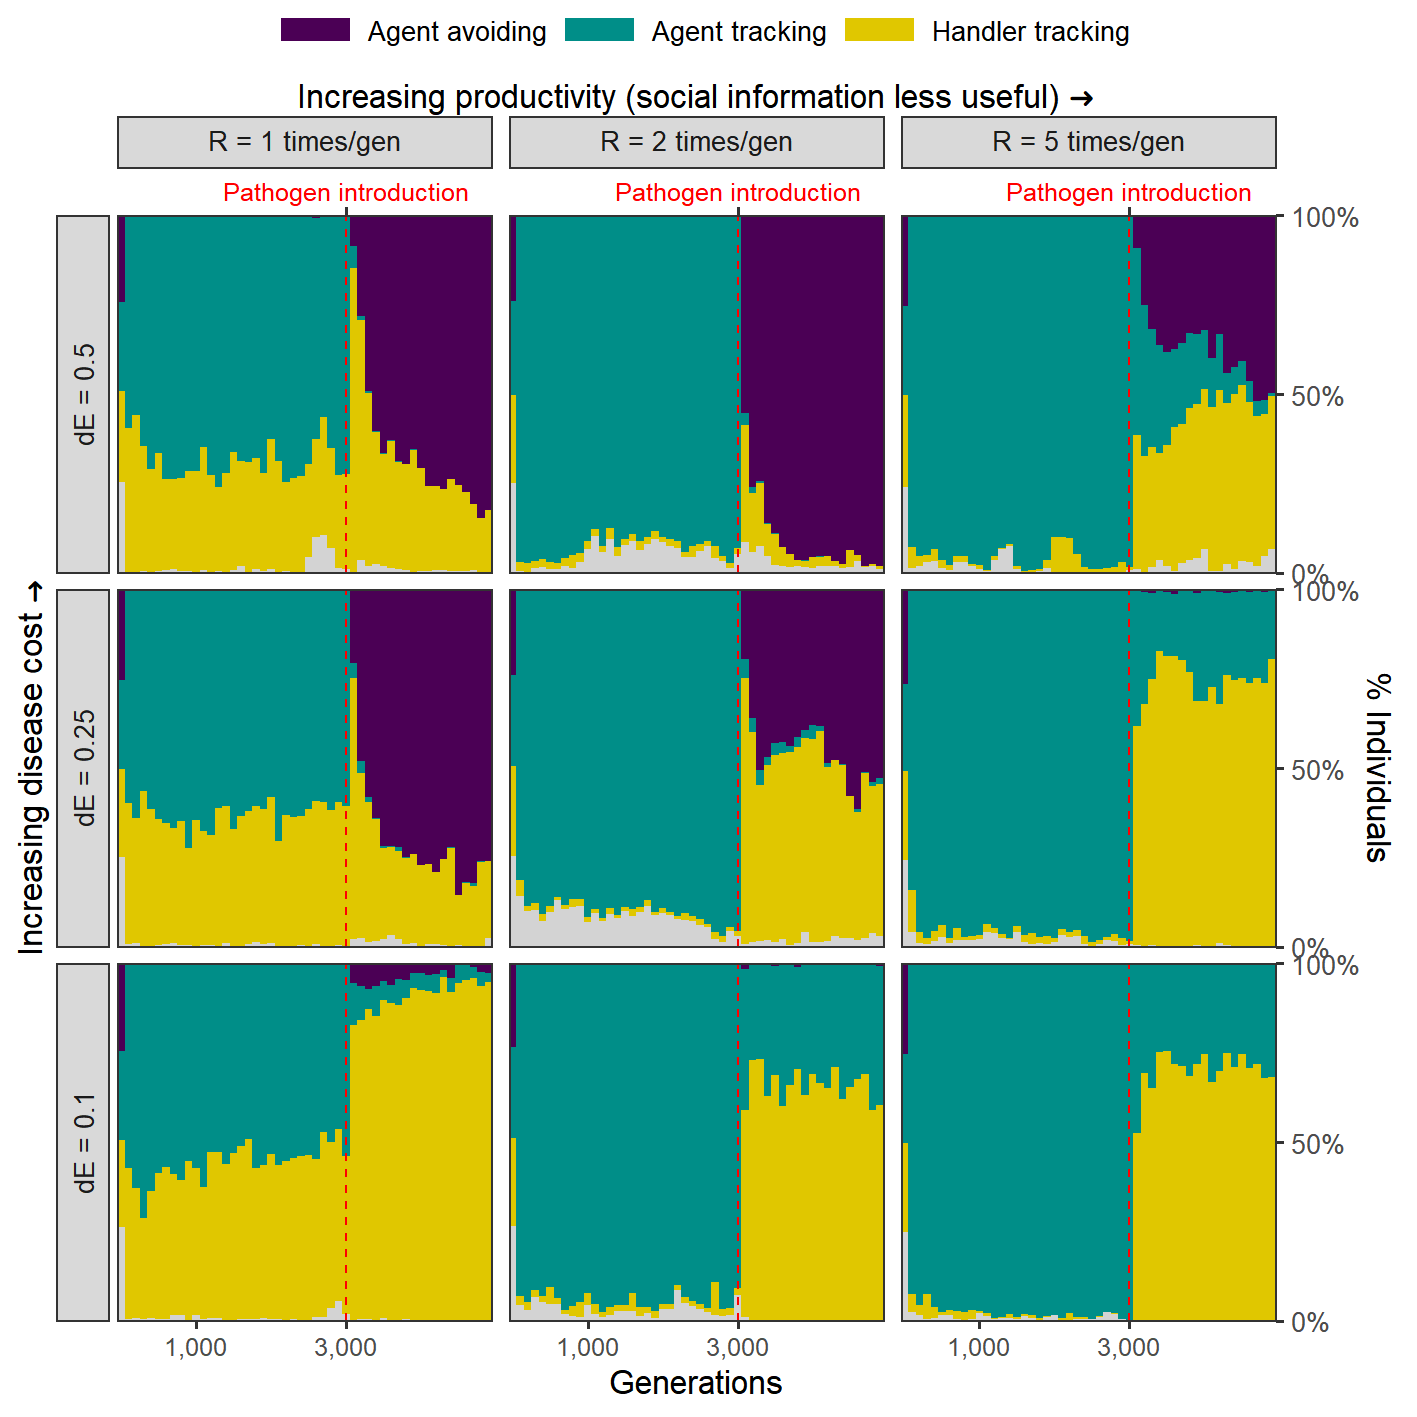
\includegraphics[width=0.8\linewidth]{figures/pathomove/fig_evo_strategy_default.png}
    % width=8.7cm
    \caption{
        \textbf{The balance of infection cost and the usefulness of social information together shape the rapid evolutionary change in movement strategies triggered by pathogen introduction.}
        Pre-introduction (G = 3,000; dashed line) populations contain a mix of individuals that either track all foragers (agent tracking), or only successful foragers (handler tracking).
        Handler tracking is more common on low-productivity landscapes (R = 1), where social information is more useful to find patchily distributed resources.
        After pathogen introduction, handler tracking rapidly becomes the most common strategy when the apparent usefulness of social information is greater than the cost of infection.
        This occurs both when productivity is low (R = 1) and infection costs are low ($\delta E$ = 0.1), but also when productivity is high (R = 5) with intermediate infection costs ($\delta E$ = 0.25).
        When the cost of infection outweighs the apparent usefulness of social information, the agent avoidance (avoiding both successful and unsuccessful foragers) emerges and rapidly becomes a common strategy ($\delta E$ = 0.5; $\delta E$ = 0.25, R = 1).
        In scenarios of high landscape productivity combined with low infection costs (e.g. R = 5, $\delta E$ = 0.1), the agent tracking strategy persists in a large proportion after pathogen introduction, as these individuals can balance disease costs with intake alone.
        All panels show mean frequencies over 10 replicate simulations in 100 generation bins; frequencies are stacked.
        Grey areas show the relatively uncommon `non-handler' tracking strategy.
    }\label{fig_evo_strategy}
\end{figure}
}

\subsection*{Usefulness of Social Information and Infection Cost Influence Evolution of Social Movement Strategies}

We further explored the effect of two ecological parameters, landscape productivity ($R \in $ 1, 2, 5) and infection cost per timestep ($\delta E \in$ 0.1, 0.25, 0.5) on simulation outcomes.
Before pathogen introduction, landscape productivity alone determines the value of social information, and thus which social movement strategies evolve (Fig.~\ref{fig_evo_strategy}).
On low-productivity landscapes (R = 1), social information is valuable as direct resource cues are scarce; here, the handler-tracking strategy persists.
On high-productivity landscapes ($R \in$ 2, 5), social information is less valuable as individuals can directly detect food items more often; here, the agent tracking strategy is most common.
Across parameter combinations, the introduction of the infectious pathogen leads to a rapid evolutionary shift in social movement strategies.
The benefits of social information, and infection cost jointly determine how pathogen introduction alters the mix of social movement strategies, but populations generally shift away from indiscriminate agent tracking, as that strategy is associated with higher infection risk (see Fig.~\ref{fig_networks_disease}A).

When the benefit of social information is equivalent to the cost of infection, the handler tracking strategy is common (R = 1, $\delta E$ = 0.1; R = 5, $\delta E$ = 0.25).
When apparent social information benefits are lower than infection costs (e.g. $\delta E$ = 0.5), the agent avoiding strategy is common.
The effect of landscape productivity in obviating a sensitivity to social information cues (especially, conspecific status) is also eroded by pathogen introduction.
On high-productivity landscapes where individuals were indiscriminately social, ($R \in$ 2, 5, $\delta E$ = 0.1), the handler tracking strategy becomes common, as individuals prioritise higher-quality social information (handlers, which indicate a resource cluster).
However, high landscape productivity can also compensate for the cost of infection, as evidenced by the agent tracking strategy remaining prevalent: this is only possible if these individuals can consume sufficient resources to overcome disease costs.

\section*{Contextualising the Outcomes of the Pathomove Model}

Our general model captures important features of infectious pathogen (or parasite) transmission among host animals in a (foraging) context that is relevant to most species.
The combination of ecological, evolutionary, and epidemiological dynamics in a spatial setting is unprecedented for movement-disease models, and 
% Our approach shows how evolution can be incorporated into mechanistic movement-disease models, and how this approach 
extends current understanding of animal spatial and social ecology \autocite{albery2021,webber2018,webber2022,romano2020,romano2021,kurvers2014}.
Presently, most movement-disease models are non-evolutionary \autocite{white2018,white2017,scherer2020,lunn2021}, presumably because evolution is expected to be too slow to impact epidemiological-ecological outcomes \autocite{monk2022}.
We demonstrate the pitfalls of this assumption: evolutionary transitions in sociality occur over fewer generations than required for the development of key aspects of animal ecology, such as migration routes \autocite{jesmer2018,cantor2021}.
We also demonstrate the tension inherent to sociality under the risk of an infectious pathogen, in an explicitly spatial context.
% We show how populations, initially evolved to find patchily distributed food using social information, rapidly evolve to become more sensitive to potential infection risk and eschew (some) social encounters, when an infectious pathogen is introduced.
Our work shows how qualitatively and quantitatively different social movement strategies --- making different trade-offs between social information and infection risk --- can co-exist in a single population \autocite{wolf2012,webber2018,gartland2021,webber2022}.

\subsection*{Social Information Use and Pathogen Introduction}

Prior to pathogen introduction, the value of social information influenced which social movement strategies were evolved. 
Individuals initialised (`born') near their parent's final location may benefit from `ecological inheritance' \autocite{badyaev2009} of their parent's favourable position near resource clusters (see \textit{SI Appendix Fig. S2, S4}).
Avoiding potential competitors (and kin) thus correlates with avoiding profitable areas, and this leads to the persistence of the indiscriminately social agent tracking strategy, despite the evident costs of exploitation competition.
In an alternative implementation with large-scale natal dispersal, handler tracking is the commonest strategy prior to pathogen introduction (see \textit{SI Appendix}).
Following pathogen introduction, the agent tracking strategy of our default scenario allows the disease to spread very easily among entire lineages of social individuals (see Fig.~\ref{fig_networks_disease}A) \autocite{kurvers2014}.
This neatly demonstrates why the risk of infection or parasitism could be among the mechanisms underlying density dependence in natal dispersal decisions \autocite{travis1999}.

Following pathogen introduction, the evolutionary shift in social movement strategies is much more rapid than the timescales usually associated with the evolution of complex traits such as sociality (about 25 generations).
Avoiding potentially infectious individuals is a key component of navigating the `landscape of disgust' \autocite{weinstein2018}.
Our results show that sensitivity to cues of high pathogen transmission risk can rapidly evolve following the introduction of a novel pathogen, with a complete replacement of the hitherto dominant social strategy.
The emergence of qualitative individual variation in social movement strategies, and especially the trade-off between movement, associations, and infection risk also demonstrates the evolution of `sociability as a personality trait' \autocite[][]{gartland2021}.

We also find substantial individual variation in the quantitative importance of social cues overall, which is a key component of the evolution of large-scale collective behaviours, such as migration \autocite{guttal2010}.
Our work suggests how, by leading to the necessary diversity in social movement strategies, a novel pathogen may actually lay the groundwork for the evolution of more complex collective behaviour.
Nonetheless, the rapid decreases in social interactions should primarily prompt concern that the evolutionary consequences of pathogen introduction could slow the transmission of, and erode, animal culture \autocite{cantor2021} --- including foraging \autocite{klump2021} and migration behaviours \autocite{jesmer2018,guttal2010}.
Pathogens themselves typically have shorter generation times than their hosts, and may also evolve rapidly in response to changes in host sociality \autocite{ashby2022}.
Although not examined here, a mixture of social strategies could allow for the maintenance of a corresponding diversity in pathogen strategies as well \autocite{ashby2022,prado2009}.

\subsection*{Ecological Causes and Consequences of Social Movement Strategies}

In our model, landscape productivity (R), is a proxy for the usefulness of sociality overall, as social information is less useful when direct resource cues are abundant (high R).
Social information benefits in disease models often have no mechanistic relationship with the subject of the information (e.g. food or predators) \autocite{ashby2022}. 
In contrast, social information benefits in our model are emergent outcomes of animal movement and foraging behaviour. 
Our predictions may help explain intra- and inter-specific diversity in social systems across gradients of infection risk and the usefulness of social information \autocite{altizer2003,sah2018}, and studies tracking social movements and potential for disease spread could form initial tests of our basic predictions \autocite{wilber2022}.
While our individuals do not die, the evolved pathogen-risk adapted, dynamic social distancing strategies \autocite{stockmaier2021} lead to a significant worsening (equivalent to a halving) of individuals' intake.
In real systems, this could increase populations' susceptibility to extreme climate change related mortality events \autocite{fey2015}.

More positively, animals may be able to adapt relatively quickly to the spillover and eventual persistence of infectious pathogens, even when they cannot specifically detect and avoid infected individuals \autocite{altizer2003,stroeymeyt2018,stockmaier2021,pusceddu2021}.
While the most noticeable effect of pathogen outbreaks is mass mortality \autocite{fey2015}, even quite serious pathogens --- Sarcoptic mange \autocite{almberg2015}, foot-and-mouth disease \autocite{jolles2021,bastos2000,vosloo2009}, SARS-CoV-2 \autocite{chandler2021,kuchipudi2022}, and avian influenza \autocite{globconsorth5n82016,wille2022} among others --- appear to spread at sub-lethal levels for many years between lethal outbreaks.
Our model shows how disease-dominated ecological cascades \autocite{monk2022} 
% --- individuals have less intake, exerting less top-down pressure on their resource --- 
could occur even without mortality effects, due to evolutionary shifts in sociality alone.
% In the \textit{SI Appendix}, we show that such a cascade occurs even when the infection costs are modelled quite differently, being considered to be a fraction of daily intake.
The altered ecological state \autocite[here, less resource consumption, as in][]{monk2022} may be maintained long after --- and indeed because --- a population has adapted to be less social in the presence of a pathogen.
Our work suggests that decreased sociality resulting from adaptation to a novel pathogen could slow the transmission of future novel pathogens. 
While decreased sociality could also reduce the prevalence of previously endemic pathogens adapted to a more social host, it may also degrade `social immunity' through reduced sharing of beneficial commensal microbes, or of low, immunising doses of pathogens \autocite{ezenwa2016,almberg2015}.

\subsection*{Feedbacks with Pathogen Chracteristics}

Our model results are contingent upon sustained introduction of the pathogen (or its novel strains) to host populations.
More sporadic introductions (once every few generations) apparently do not cause evolutionary shifts in social movement (\textit{SI Appendix}).
Yet repeated pathogen and parasite introductions among susceptible populations appear to be quite common \autocite{levi2012,jolles2021,vosloo2009,bastos2000,scherer2020,globconsorth5n82016,wille2022}.
Such introductions are often detected only among easily observed groups such as birds \autocite{wille2022}, or after evident mass mortality events \autocite{fey2015,fereidouni2019}.
Seasonal host-pathogen dynamics could and do keep pathogens circulating in reservoir hosts, with regular pulses in primary infections similar to our model (e.g. due to new calves in African buffalo hosting foot-and-mouth disease: \cite{jolles2021}, or winter peaks in mange among wolves: \cite{almberg2015}).
Existing host-pathogen dynamics, and potential pathogen range expansions, could thus provide more frequent opportunities for novel transmissions to overlapping species than previously guessed.
Our model shows how this provides a powerful selective force in favour of detecting and avoiding infection risk cues \autocite{weinstein2018}.

Pathogens also typically have much shorter generation times than their hosts.
Analytical models expect pathogen attributes to rapidly co-evolve to match host population attributes (e.g. sociality and immune resistance) \citep[][]{bonds2005,prado2009,ashby2022}.
Such models treat pathogens --- just as they do host animals --- in relatively simple, non-mechanistic ways.
Pathogens are primarily expected to evolve to a virulence that promotes between-host transmission \citep{bonds2005}.
Our mechanistic model does not explicitly consider host-pathogen co-evolutionary dynamics, as this complexity was beyond the scope of our general, conceptual model.
Adding pathogen evolutionary dynamics to a mechanistic individual-based model would require careful consideration of \textit{(i)} the costs the pathogen imposes on its hosts, and \textit{(ii)} how it transmits between hosts, both within and between generations.
We expect that multiple pathogen strategies could coexist in a host population that itself has multiple social movement strategies.

\subsection*{Towards Hypothesis-testing and Predictive Modelling}

In order to be widely applicable to diverse novel host-pathogen introduction scenarios, our model is necessarily quite general.
A wide diversity of pathogens and their dynamics remains to be accurately represented in individual-based models \autocite{white2017,white2018,scherer2020,lunn2021}. 
Our framework can be expanded and specifically tailored to real-world situations in which populations are repeatedly exposed to novel pathogens (or strains) \autocite{scherer2020,wille2022,bastos2000,jolles2021,chandler2021,kuchipudi2022}.
Such detailed implementations could include aspects of the pathogen life-cycle \autocite{white2018a,white2017}, account for sociality as a counter to infection costs \autocite{ezenwa2016,almberg2015}, or model host-pathogen sociality-virulence co-evolution \autocite{ashby2022,prado2009,bonds2005}.
We generate consistent predictions of marked and swift evolutionary shifts in social movement strategies that could plausibly be tested over the timescales of some long-term animal tracking studies \citep{wilber2022}.

Importantly, our social information-based movement strategies are made up of continuous values that place individuals on a two-dimensional trait space of relative preferences (or aversions) for successful and unsuccessful foragers (see \textit{Model and Analysis}; \cite{bastille-rousseau2019}).
Such social movement strategies could already be revealed for free-living animals using newer step-selection approaches \citep{avgar2016}, combined with the simultaneous, high-throughput tracking of many hundreds of animals in an area \citep{nathan2022}.
Future work would ideally combine wildlife monitoring and movement tracking across gradients of pathogen prevalence, to detect novel cross-species spillovers \autocite{chandler2021,kuchipudi2022} and study the spatial and epidemiological consequently of animal movement strategies \autocite{bastille-rousseau2019,wilber2022,monk2022}.
Given that infection patterns can change rapidly in space even in small, well-mixed populations \citep{albery2022}, the systems that could be used to test these phenomena may be widespread and easily available.
Finally, our model shows why it is important to consider evolutionary responses in movement-disease studies, and provides a general framework to further the integration of evolutionary approaches in wildlife spatial epidemiology.

% \subsection*{Data and Code Availability}

% The \textit{Pathomove} simulation model code is available on Zenodo at https://zenodo.org/record/6331816, and on Github at github.com/pratikunterwegs/pathomove.
% A reference dataset with 10 replicates of the parameter combinations presented here is archived on Zenodo at: https://zenodo.org/record/6331757.
% Code to run the simulations and analyse the output is on Zenodo at https://zenodo.org/record/6341440, and on Github at: 
% github.com/pratikunterwegs/patho-move-evol.

% \subsection*{Acknowledgements}
% We thank Jan Kreider for helpful feedback on an early draft of the manuscript;
% and Thijs Janssen for help with the simulation model code.
% We thank the Center for Information Technology of the University of Groningen for providing access to the \textit{Peregrine} high performance computing cluster to run simulations.
% P.R.G was supported by an Adaptive Life Programme grant made possible by the Groningen Institute for Evolutionary Life Sciences (GELIFES).
% J.G. was supported by a grand from the Netherlands Organization for Scientific Research (NWO-ALW; ALWOP.668).
% F.J.W. acknowledges funding from the European Research Council (ERC Advanced Grant No. 789240).

{ \begin{center} \barfont{-.-} \end{center} }

\newpage

\begingroup

\let\clearpage\relax
\let\cleardoublepage\relax
\let\cleardoublepage\relax

{\chapter*{Supplementary Information for Chapter~\ref{ch:pathomove}}}

\begin{figure}[!h]
    \centering
    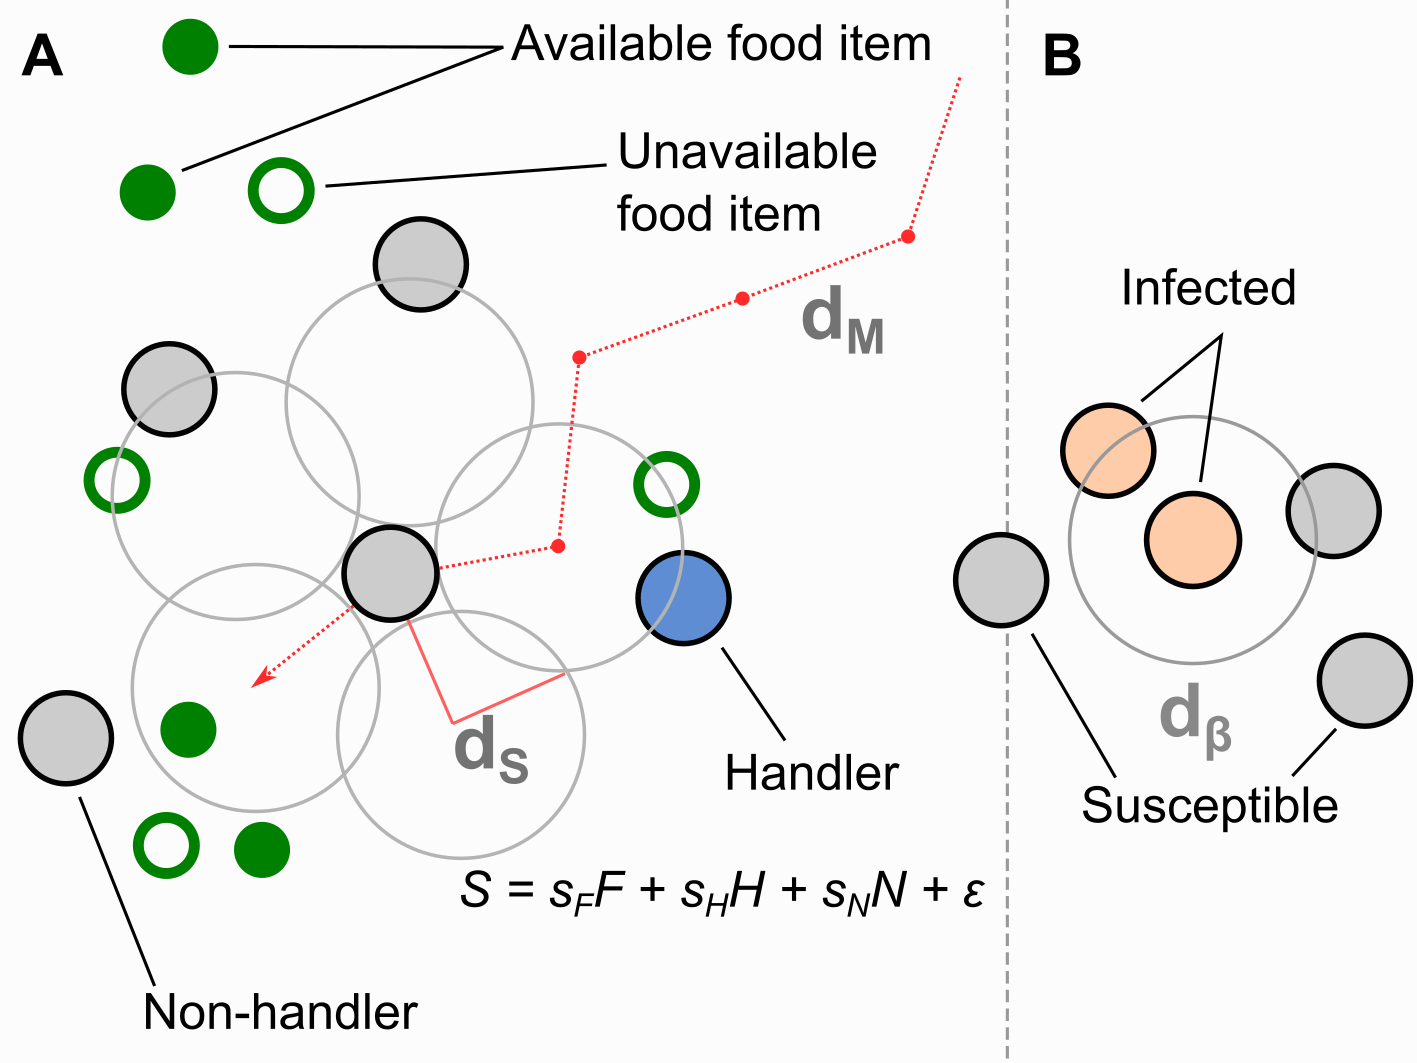
\includegraphics[width=0.75\textwidth]{figures/pathomove/fig_schematic.png}
    \caption{
        \textbf{Model implementation of discrete movement steps in continuous space, with movement steps selected based on inherited preferences for environmental cues.} 
        In our model, \textbf{(A)} individuals search for food items (\textbf{green circles}), which may be immediately available (\textbf{filled green circles}; \emph{F}), or may be available only in the future (\textbf{open green circles}). 
        Individuals can sense only available items, and not unavailable ones. However, given our landscape structure, food items are clustered, making available items a good indicator of where resource clusters are (see next figure). 
        Individuals can also sense other foraging individuals, and can sense whether they have successfully found, and are handling, a food item (handlers; \textbf{blue circles}), or whether they are unsuccessful foragers still searching for food (non-handlers; \textbf{filled grey circles}; \emph{N}). 
        To decide where to move, individuals sample their environment for these three cues (\emph{F, H, N}) at 5 locations around themselves (\textbf{large open grey circles}), and have a sensory range of \(d_S\). 
        When the sensory range is relatively large (default = 1.0 units), there is some small overlap in samples. 
        Individuals assign each potential direction a \emph{suitability}, \(S = s_FF + s_HH + s_NN + \epsilon\), where the coefficients \(s_F, s_H, s_N\) are inherited preferences for environmental cues, and \(\epsilon\) is a small error term that helps break ties between locations. 
        In our implementation, the sensory distance (\(d_S\)) and the movement distance (\(d_M\)) are the same, 1.0 units. 
        \textbf{(B)} Our infectious pathogen is transmitted between infected (\textbf{orange circles}) and susceptible (\textbf{filled grey circles}) individuals, with a probability \(p\) = 0.05, when they are within a distance \(d_\beta\) of each other. 
        In our implementation, \(d_\beta\) is the same as \(d_S, d_M\) = 1.0 units.
    }\label{fig:patho_schematic}
\end{figure}

\begin{figure}
    \centering
    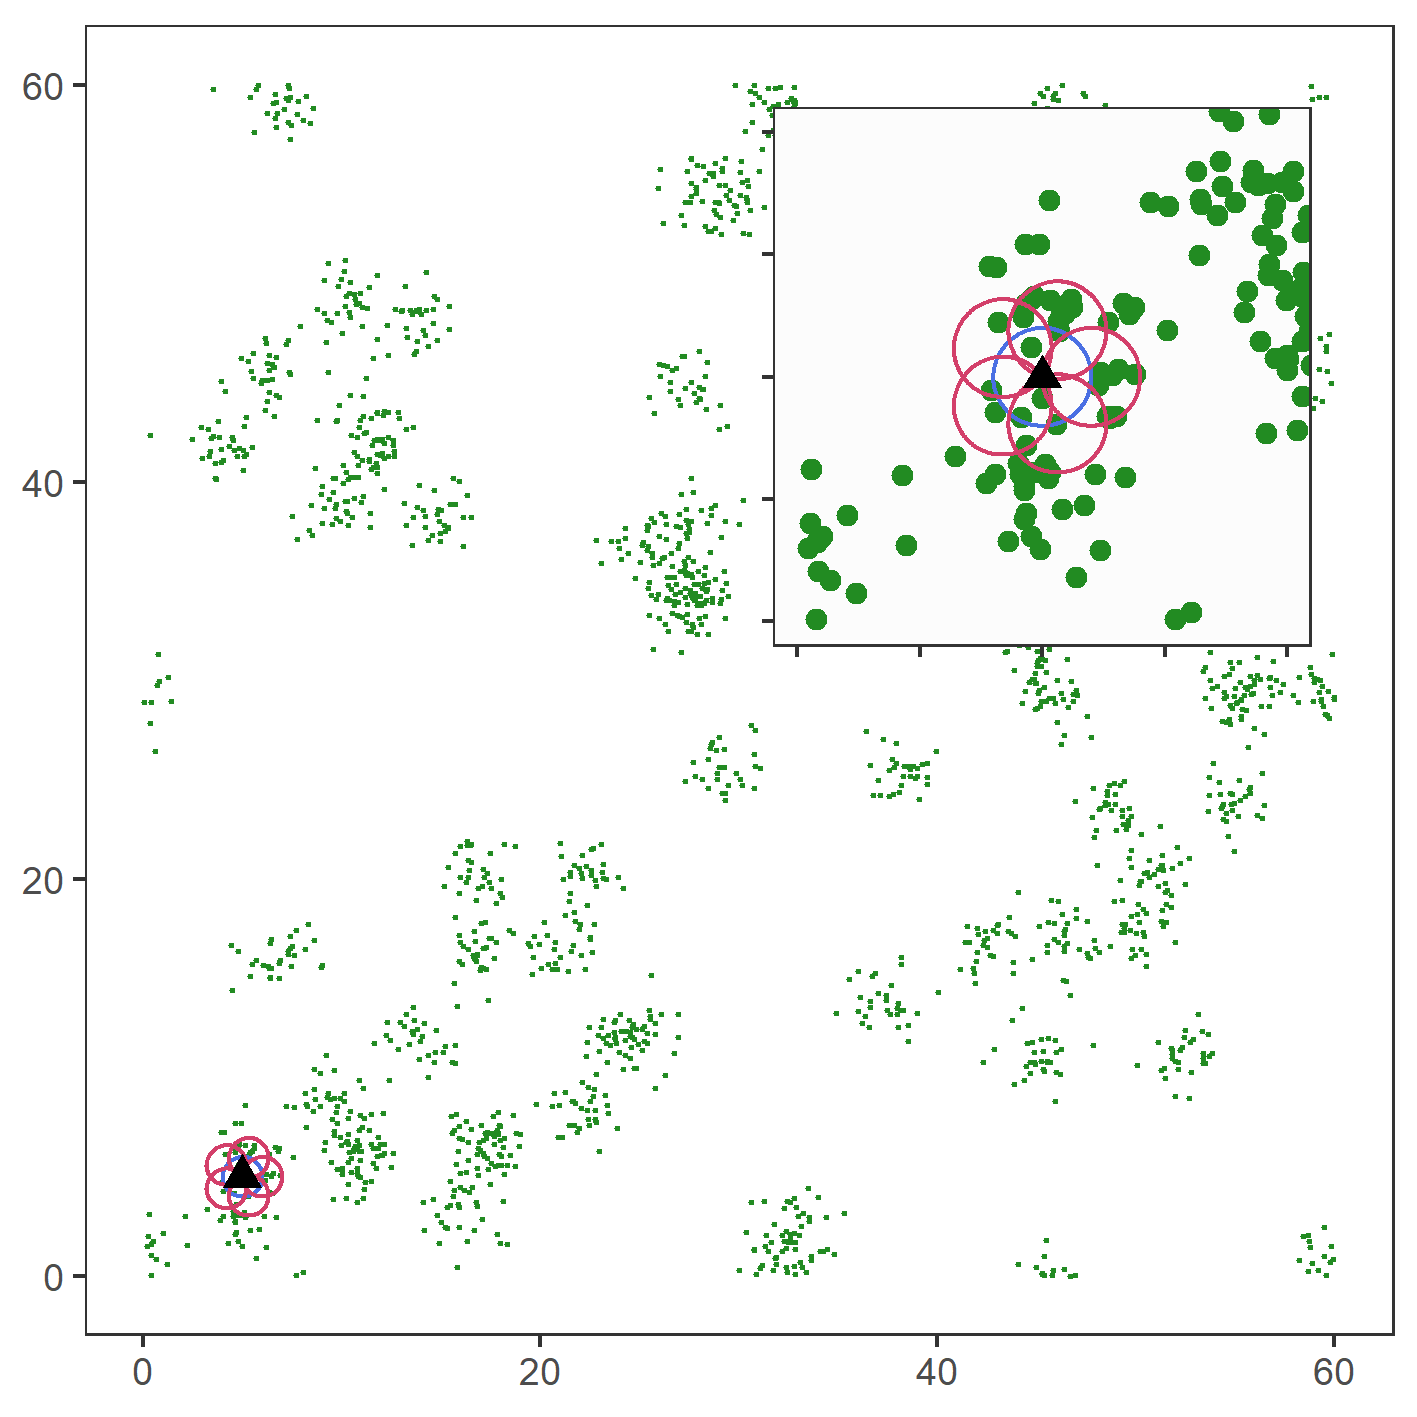
\includegraphics[width=0.7\textwidth]{figures/pathomove/fig_landscape.png}
    \caption{
        \textbf{An example of the resource landscape used in our simulations.} 
        Our simulation's resource landscape consists of 60 randomly distributed clusters of food items (`resource patches'), with 1800 discrete food items divided among the clusters (30 items per cluster). 
        The landscape is a square of 60 units per side, with wrapped boundaries (i.e., a torus). 
        The food item density in our scenarios is 0.5 food items per unit area. 
        Items are distributed around the centre of each cluster, within a standard deviation of 1.0 unit. 
        Items, once consumed by foragers, are unavailable for a fixed number of timesteps (the regeneration time $R$, expressed in terms of the foragers' generation time), after which they regenerate in the same location. 
        While regenerating (i.e., unavailable). While regenerating, items cannot be sensed by foragers. 
        The sensory ranges of individuals (\(d_S\)) are shown for each potential step (\textbf{red circles}, including the current location: \textbf{blue circle}). 
        Food item clustering means that available items, as well as foragers handling a food item (handlers) are good indicators of the location of a resource cluster.
    }\label{fig:patho_landscape}
\end{figure}

\begin{figure}
    \centering
    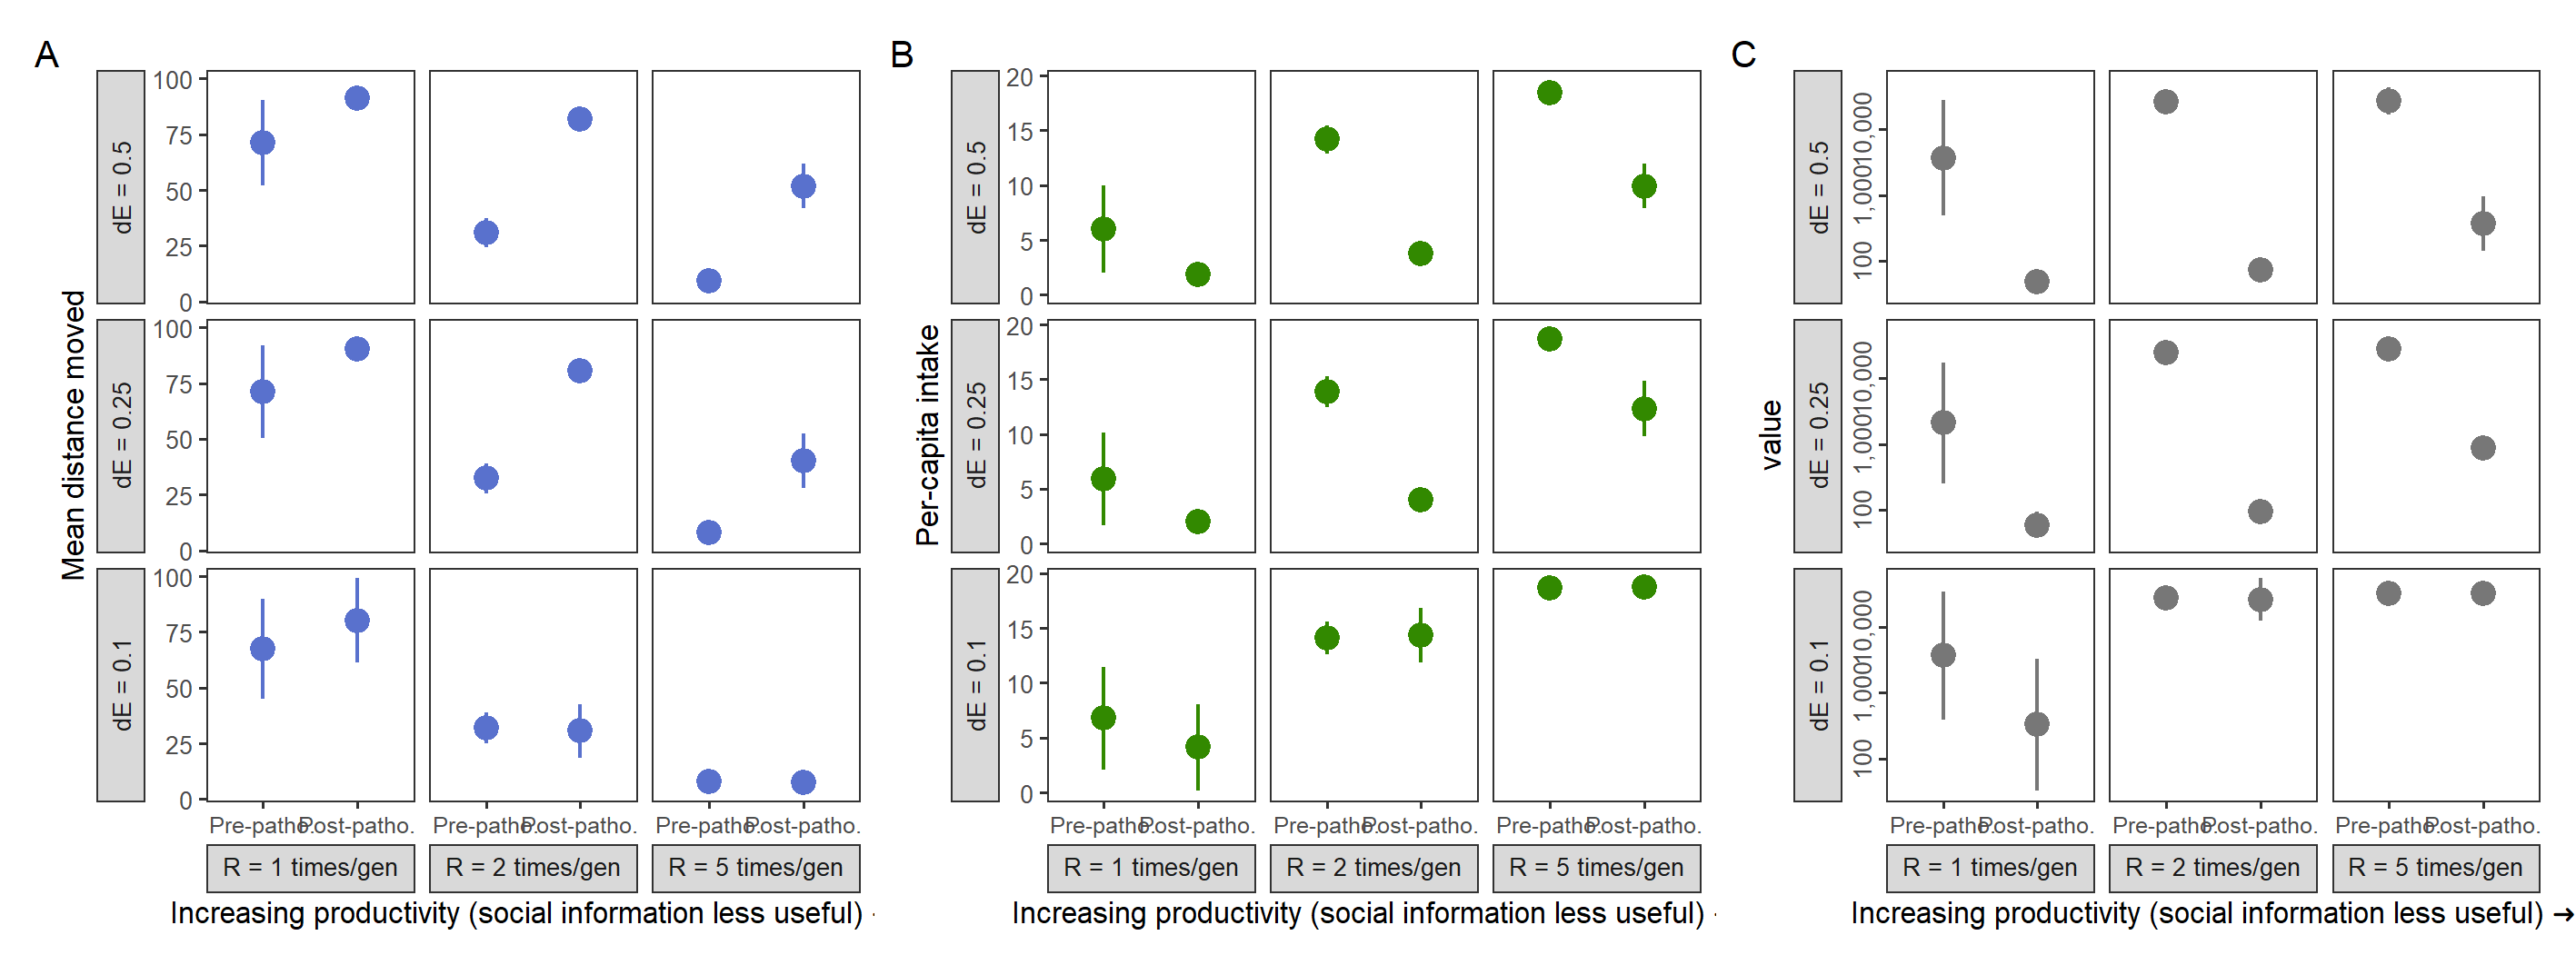
\includegraphics[width=0.95\textwidth]{figures/pathomove/fig_eco_compare_default.png}
    \caption{
        \textbf{Rapid changes in ecological outcomes following pathogen introduction.} 
        The introduction of the infectious pathogen leads to rapid evolutionary changes in movement strategies (see Figures 1 and 5; main text) across most combinations of landscape productivity and infection cost. 
        In all combinations where there is rapid evolutionary shift in social-movement strategies, there is a similar change in the population's ecological outcomes: more movement, less intake, and fewer associations. 
        Only in scenarios where the mix of social-movement strategies does not change (\(R \in\) 2, 5; $\delta~E$ = 0.1), is there broadly no change in population ecological outcomes. 
        Each subplot in each panel shows the mean and standard error of the per-capita values for \textbf{(A)} distance moved, \textbf{(B)} intake, \textbf{(C)} number of associations, or encounters, with other individuals. 
        Means and standard deviations are shown before (G = 3,000) and after (G = 3,500) pathogen introduction; each data point represents 10 replicates of the relevant parameter combination.
    }\label{fig:patho_eco_compare}
\end{figure}

\section*{Effect of Modelling Choices}

Modelling choices can have a substantial effect on the outcomes of simulations with multiple, complex interactions among components \parencite{scherer2020,gupte2021a,netz2021}.
We show the effect of varying implementation on two key aspects of our model: \textit{(1)} where individuals are initialised, or `born', on the landscape (natal dispersal), \textit{(2)} how the infectious pathogen imposes fitness costs.

\subsection*{Global Natal Dispersal of Individuals}

Some models initialise the individuals in each new generation at random locations on the landscape (see e.g. \cite*{gupte2021a}; Chapter~\ref{ch:kleptomove}); this can be called `global' natal dispersal.
This is a reasonable choice when modelling animals during a specific stage of their life cycle, such as after arriving on a wintering or breeding site after migration.
Our default choice, on the other hand, is `local' natal dispersal, where individuals are initialised close to their parent's last position.
This is also defensible, as many organisms do not disperse very far from their ancestors.
When animals do not disperse very far, they may not evolve movement rules that can be generalised across all landscape conditions, especially when the landscape is ecologically heterogeneous.
Instead, animals may adapt their strategies to the local conditions which they inherit from their parents ({`ecological inheritance'}; \cite{badyaev2009}).

Successful individuals are likely to have more offspring than unsuccessful individuals, and successful individuals are likely to be found --- in our simulation and in real natural systems --- on or near profitable resource patches.
This means that many individuals are initialised near profitable patches.
In this case, and because of the sparse distribution of resource patches on the landscape, individuals adapt to tolerate their many neighbours (who are often kin), as avoiding them would lead to also moving away from a profitable patch.

By forcing animals in each new generation to encounter ecological circumstances potentially different from those of their parents, implementing global dispersal can help investigate whether animals' evolved movement strategies are truly `optimal' at the global scale.
We implementated global dispersal by running 10 replicates of each parameter combination (9 combinations of $\delta~E$ and $R$; 90 simulations in all), with dispersal set to 10.
This means that individuals' initial positions are drawn from a normal distribution with standard deviation = 10, centred on the location of their parent (see Fig.~\ref{fig:patho_dispersal}; blue circles).

\begin{figure}
    \centering
    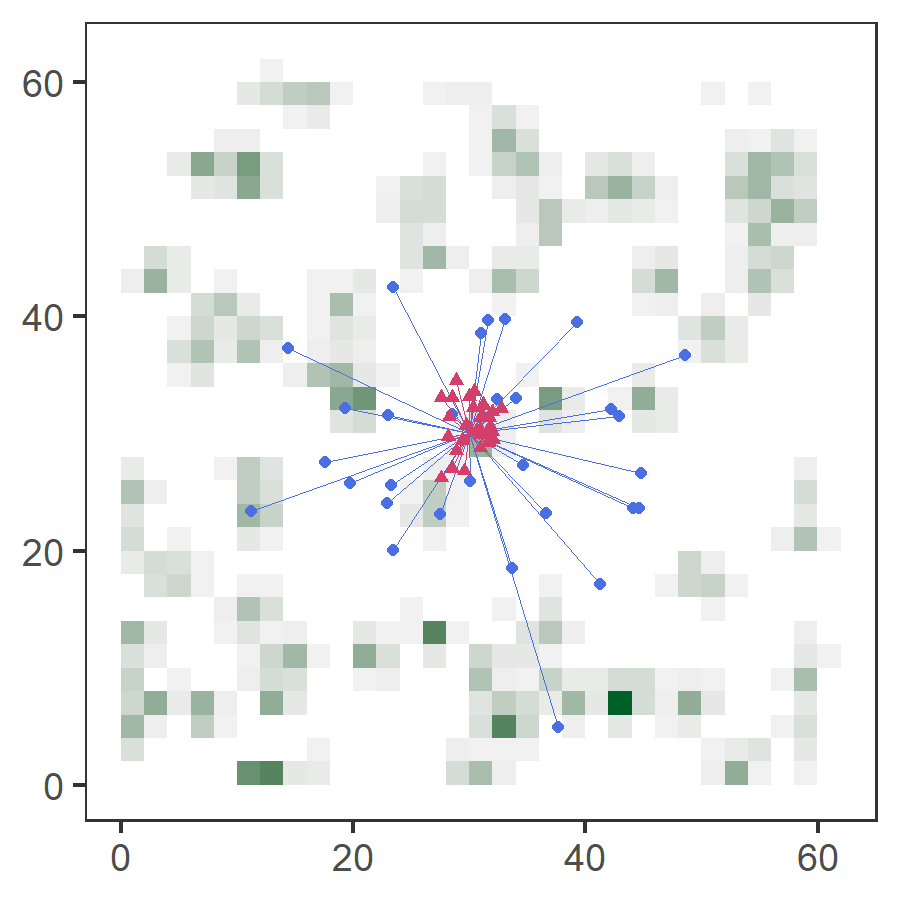
\includegraphics{figures/pathomove/fig_global_dispersal.png}
    \caption{
        \textbf{Differences between local and global dispersal.} 
        Initialising individuals in each new generation within a standard deviation of 10 units around their parent (\textbf{blue}; parent at [30, 30]) places can lead them to encounter potentially very different ecological, and social, circumstances from those of their parent. In contrast, individuals initialised close to their parents (within a standard deviation of 2 units; \textbf{red}) encounter very similar conditions as their parent. The latter also leads to substantial competition among kin. We used 10 units to represent (nearly) global dispersal, and 2 units to represent local dispersal; this is controlled by the simulation parameter \emph{dispersal}, which takes a numeric argument.
    }\label{fig:patho_dispersal}
\end{figure}

\subsection*{Evolutionary Outcomes of the Global Dispersal Implementation}

In the global dispersal scenario (see Fig.~\ref{fig:patho_dispersal}), there is a marked difference in which social movement strategy is evolved before pathogen introduction.
Since individuals are initialised relatively far away from their parent's position, they encounter potentially very different ecological conditions, both in terms of the number of other individuals, and the local availability of food items.

As a result, most individuals evolve a `handler tracking' social movement strategy before the introduction of the novel pathogen.
This strategy allows individuals to gain the benefits of social information on the location of a resource patch (of which handlers are an indirect cue), while avoiding potential competitors, as well as potentially moving away from areas without many food items.

After pathogen introduction, there is a rapid evolutionary shift in social movement strategies, similar to the shift seen in our default implementation of local dispersal.
However, these shifts only occur under conditions where the cost of infection is apparently greater than the value of using social information to find food items.
In brief, \emph{(1)} when the benefits of social information cannot compensate for the costs of infection risk ($\delta E$ = 0.5; $\delta E$ = 0.25, and R = 1, 2), the agent avoiding strategy becomes more prevalent, similar to the local dispersal case. \emph{(2)} When the costs of infection are lower than the benefits of social information, or when the resource landscape's productivity can offset the cost of infection, the handler tracking strategy persists as the dominant strategy (see Fig.~\ref{fig:patho_evo_global}).

\begin{figure}
    \centering
    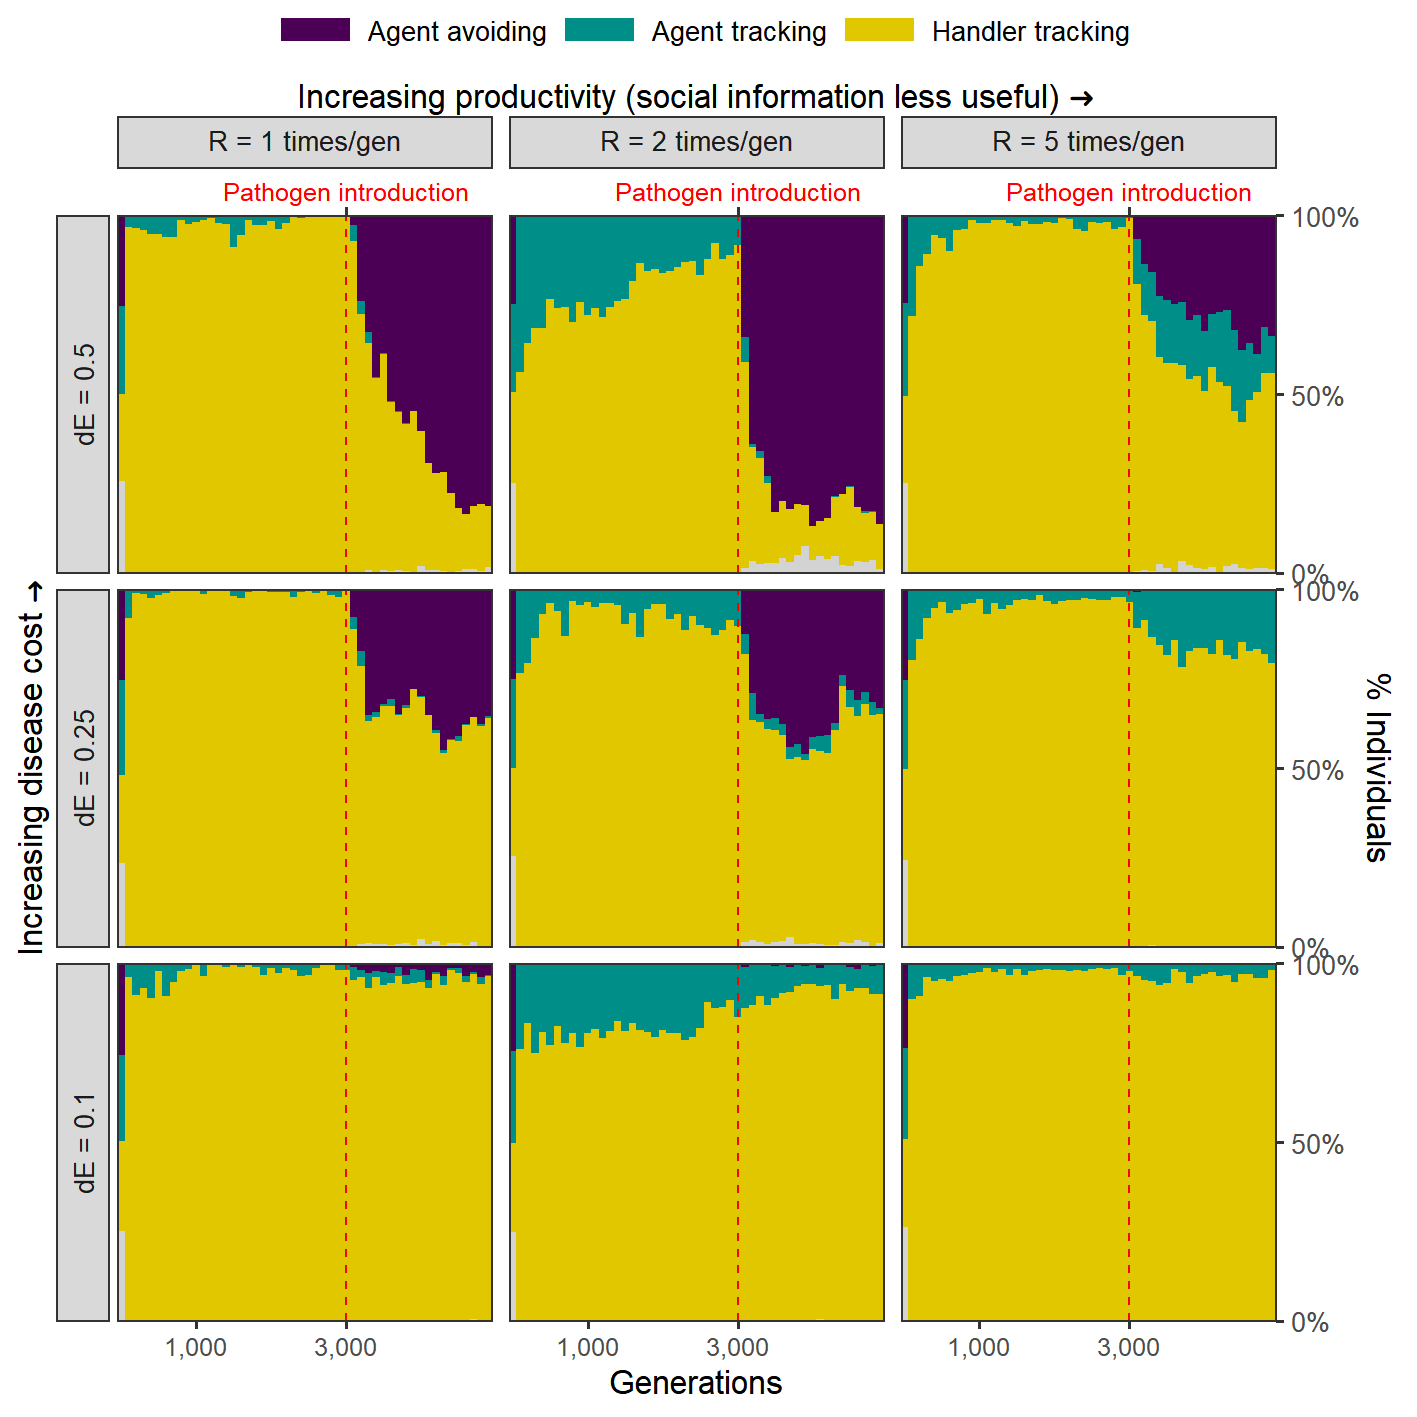
\includegraphics[width=0.9\textwidth]{figures/pathomove/fig_evo_change_global_dispersal.png}
    \caption{
        \textbf{Pathogen introduction triggers similar evolutionary changes under global dispersal as under local dispersal.} In our alternative, global natal dispersal implementation, the handler tracking strategy is the dominant strategy across most parameter combinations prior to pathogen introduction. Following pathogen introduction, there is a rapid shift in the mix of movement strategies under some ecological conditions. When the cost of infection is greater than the apparent benefit of social information, the agent avoiding strategy becomes more common. When infection costs are low ($\delta E$ = 0.1), pathogen introduction does not alter the mix of movement strategies, and the handler tracking strategy continues to be the most common strategy.}
    \label{fig:patho_evo_global}
\end{figure}

\subsection*{Ecological Consequences in the Global Dispersal Implementation}

In the global dispersal implementation, there is little to no change in population-level ecological outcomes --- mean distance moved, mean per-capita intake, and the mean number of associations --- following pathogen introduction (Fig.~\ref{fig:patho_global_eco}).
This is despite the drastic shift in evolved social movement strategies.
This is likely because a large part of individual's lifetimes (at low $R$, up to 90 timesteps), are spent moving, likely to find resource clusters.
Since intake depends on finding these clusters, and associations mostly take place at or near resource clusters, these are also reduced compared to our local dispersal implementation.

\begin{figure}
    \centering
    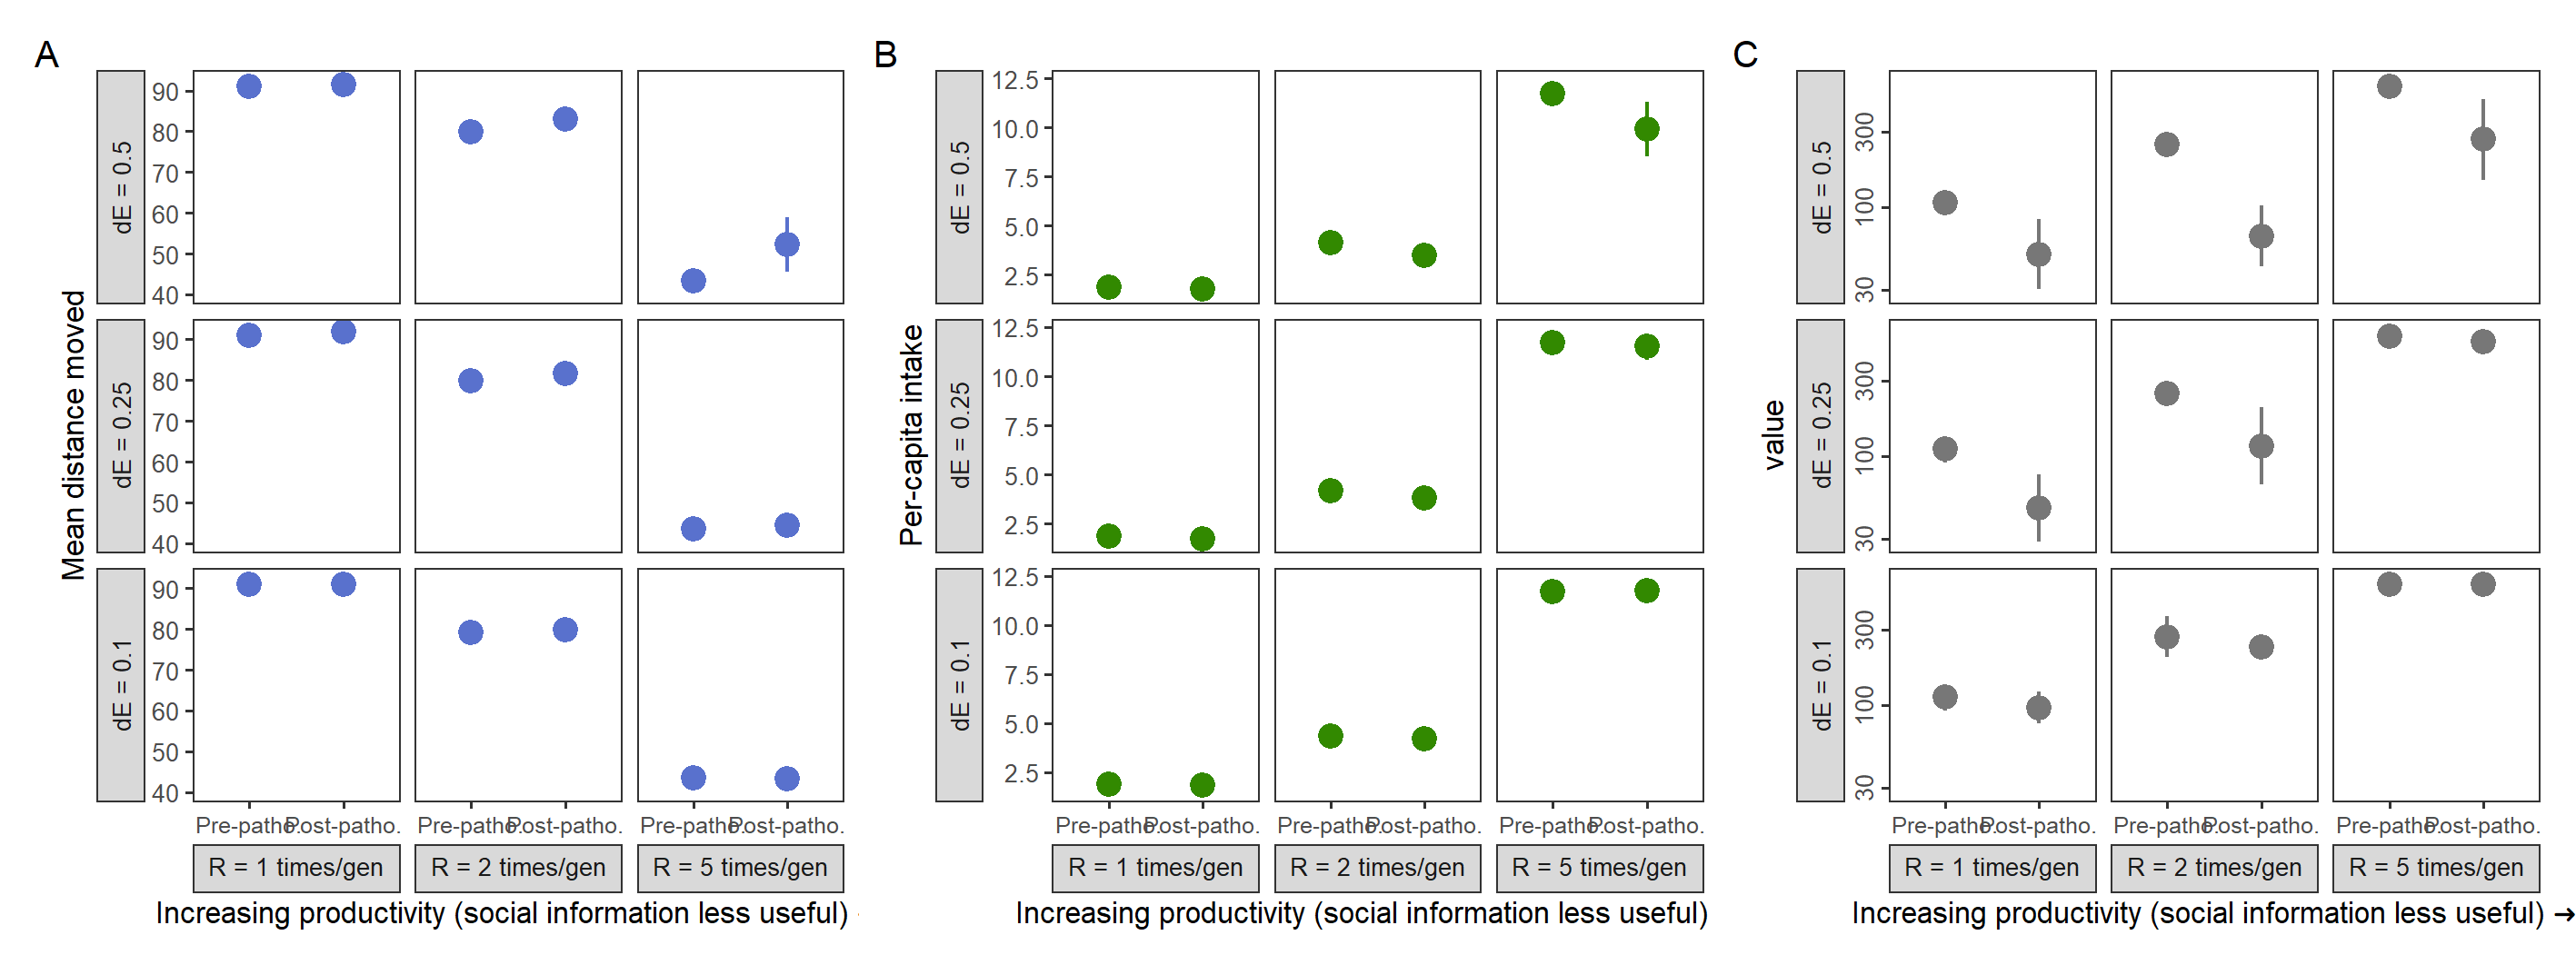
\includegraphics[width=0.95\textwidth]{figures/pathomove/fig_eco_compare_global.png}
    \caption{
        \textbf{Little to no change in ecological outcomes when implementing global dispersal.} Despite strong and rapid evolutionary shifts in social movement strategies, the ecological outcomes for populations with global natal dispersal are very similar before and after the introduction of the infectious pathogen. Each subplot in each panel shows the mean and standard error of the per-capita values for \textbf{(A)} distance moved, \textbf{(B)} intake, \textbf{(C)} number of associations, or encounters, with other individuals. Means and standard deviations are shown before (G = 3,000) and after (G = 3,500) pathogen introduction; each data point represents 10 replicates of the relevant parameter combination.
    }\label{fig:patho_global_eco}
\end{figure}

\subsection*{Infection Cost as a Percentage of Intake}

In our model's default implementation, the infectious pathogen imposes a direct cost, $\delta~E$, on individuals, in each timestep that they are infected.
For an individual with intake $N$, the net energetic gain $E$ after being infected by a pathogen for $t$ timesteps is $E = N - (\delta E \times t)$.
In this scenario, \emph{infection costs are independent of intake}.

In an alternative implementation, the infectious pathogen may be considered to reduce an animal's ability to process intake, or to require a portion of daily intake to resist.
Such an implementation is used in \ldots{}
For an individual with intake $N$, the net energetic gain $E$ after being infected by a pathogen for $t$ timesteps is $E = N \times (1 - \delta E) ^ t$.
Naturally, the two cost structures are not easy to compare, but a comparison of the potential outcomes is shown in Fig.~\ref{fig:compare_cost_structure}.

\begin{figure}
    \centering
    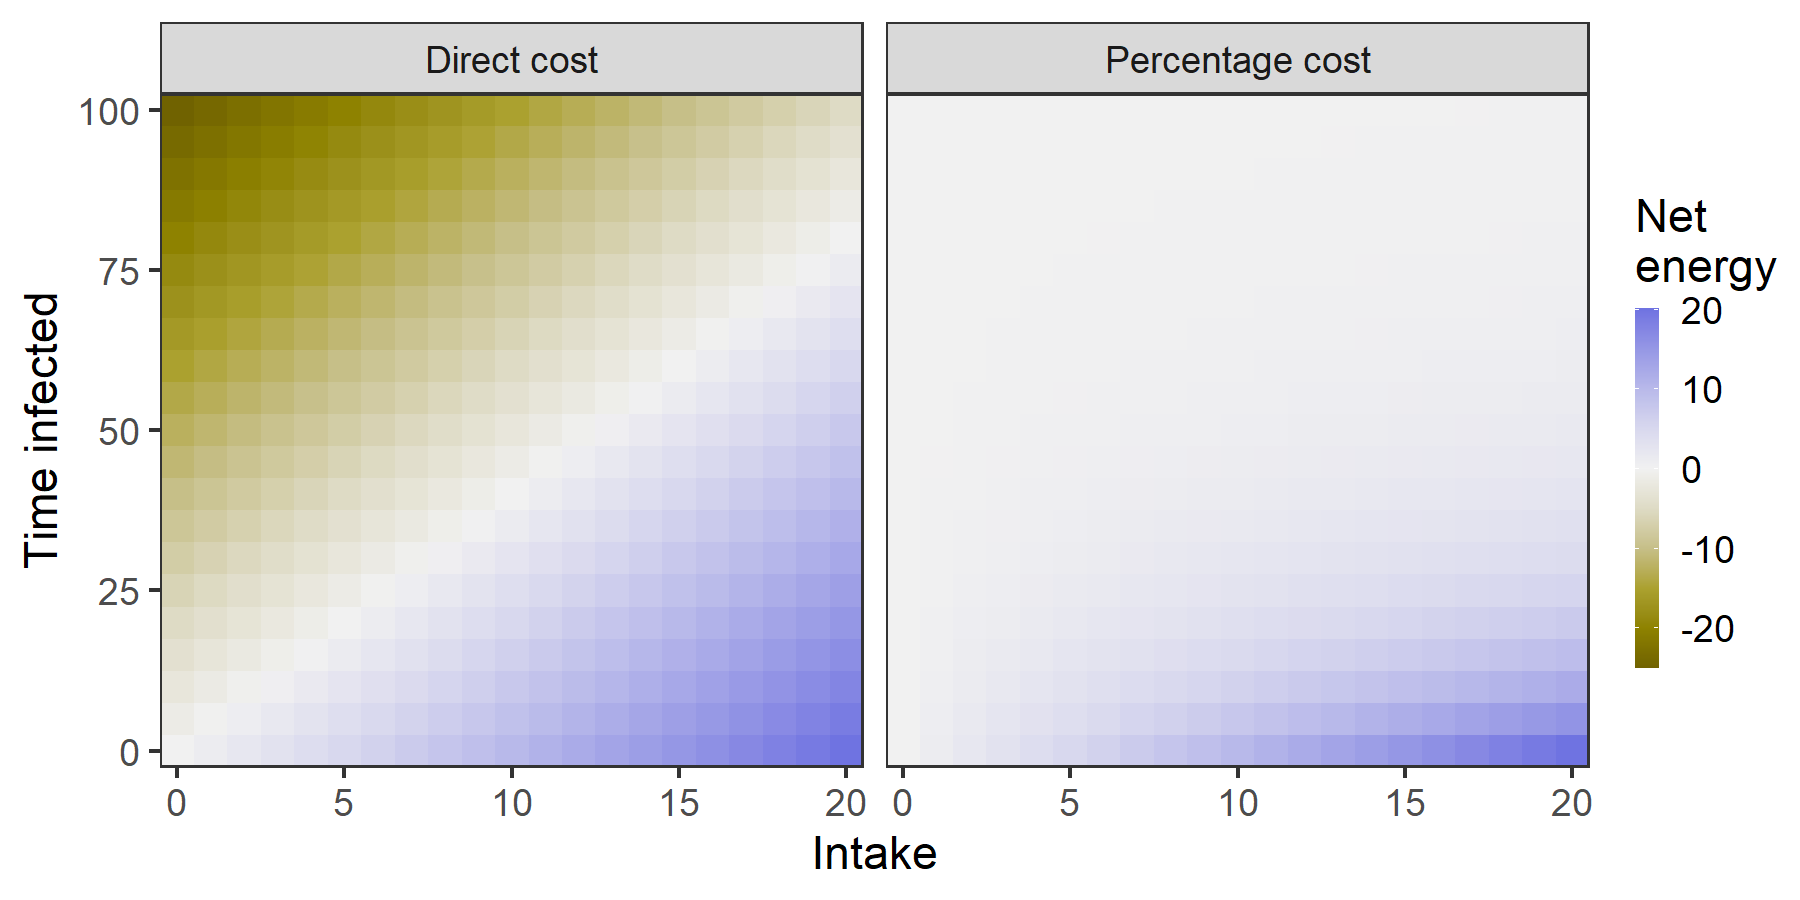
\includegraphics[width=0.7\textwidth]{figures/pathomove/fig_cost_structure.png}
    \caption{
        Calculated net energy for different combinations of intake and time infected. 
        In the \emph{Direct cost} scenario, and with a $\delta~E$ of 0.25 (shown here), which is our default implementation, an individual foraging on an item (handling time = 5 timesteps) would gain 1.0 unit of intake, and lose 1.25 units of energy in that same period if it were infected, for a net energy balance in that period of -0.25. 
        Individuals' energetic balance is normalised (0 -- 1) with reference to the lowest value in each generation. 
        Here, individuals' infection cost is \emph{independent} of their intake. 
        In the \emph{percentage cost} scenario, individuals' infection costs are linked to their intake. 
        For a per-timestep 5\% loss of intake (shown here), individuals infected for $>$25 timesteps already have a net energy balance close to, but never less than, zero. 
        In this implementation, individuals' energy balances are \emph{not normalised} with reference to the lowest net energy, as no individual's energy is ever less than zero.
    }\label{fig:compare_cost_structure}
\end{figure}

\subsection*{Evolutionary Outcomes of the Percentage Cost Implementation}

The social movement strategies evolved prior to pathogen introduction are identical to those seen in our default implementation.
This is because the percentage cost implementation differs from the default only after the pathogen is introduced.
After pathogen introduction, there is a rapid evolutionary shift in movement strategies.
This shift is similar to that in our default implementation, but the strategies evolved are different.
The handler tracking strategy becomes common across parameter combinations.
However, when the costs of infection are relatively high (7.5\%), and the usefulness of social information is limited by the abundance of food items (R = 5), the agent avoiding strategy forms about one fourth of the population mixture of social movement strategies

\begin{figure}
    \centering
    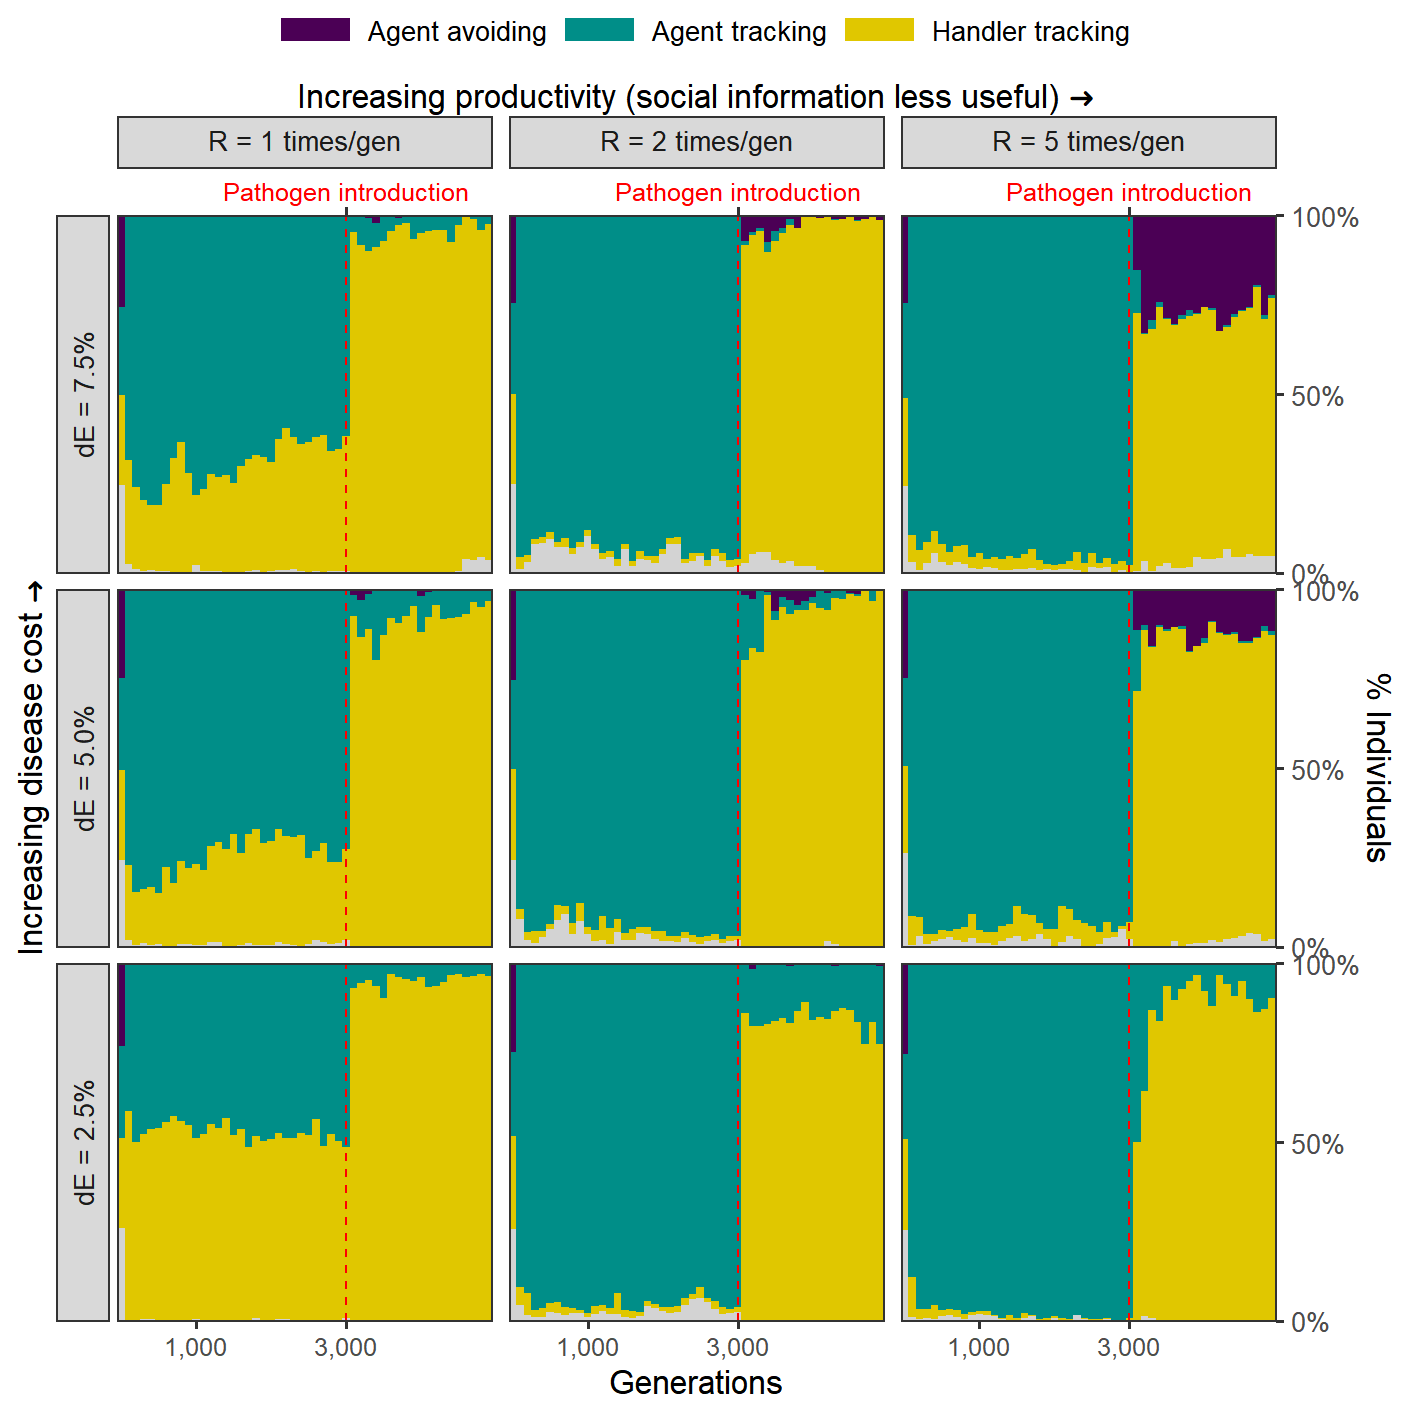
\includegraphics[width=0.9\textwidth]{figures/pathomove/fig_evo_change_percent_cost.png}
    \caption{
        \textbf{Rapid evolutionary change, but different evolutionary outcomes, in an alternative implementation of disease costs.} In our alternative, percentage costs implementation of the infectious pathogen, there is a rapid shift in the mix of movement strategies after pathogen introduction. The handler tracking strategy becomes common across all parameter combinations. Only when the costs of infection are relatively high (7.5\%), and the usefulness of social information is limited by the abundance of food items (R = 5), does the agent avoiding strategy form about one fourth of the population mixture of social movement strategies.
    }
\end{figure}

\subsection*{Ecological Consequences in the Percentage Cost Implementation}

Surprisingly, the implementation of a different cost structure for the novel, infectious pathogen does not affect ecological, population level outcomes when compared with outcomes in our default implementation of direct costs.
Across parameter combinations where there is a rapid evolutionary transition from agent tracking to handler tracking as the dominant strategy, there is also an increase in distance moved, a reduction in intake, and a reduction in associations.
Notably, the reductions in per-capita intake following pathogen introduction are similar to a halving of landscape productivity (as in the default implementation), and there is a comparable drop in the number of pairwise associations among individuals.

\begin{figure}
    \centering
    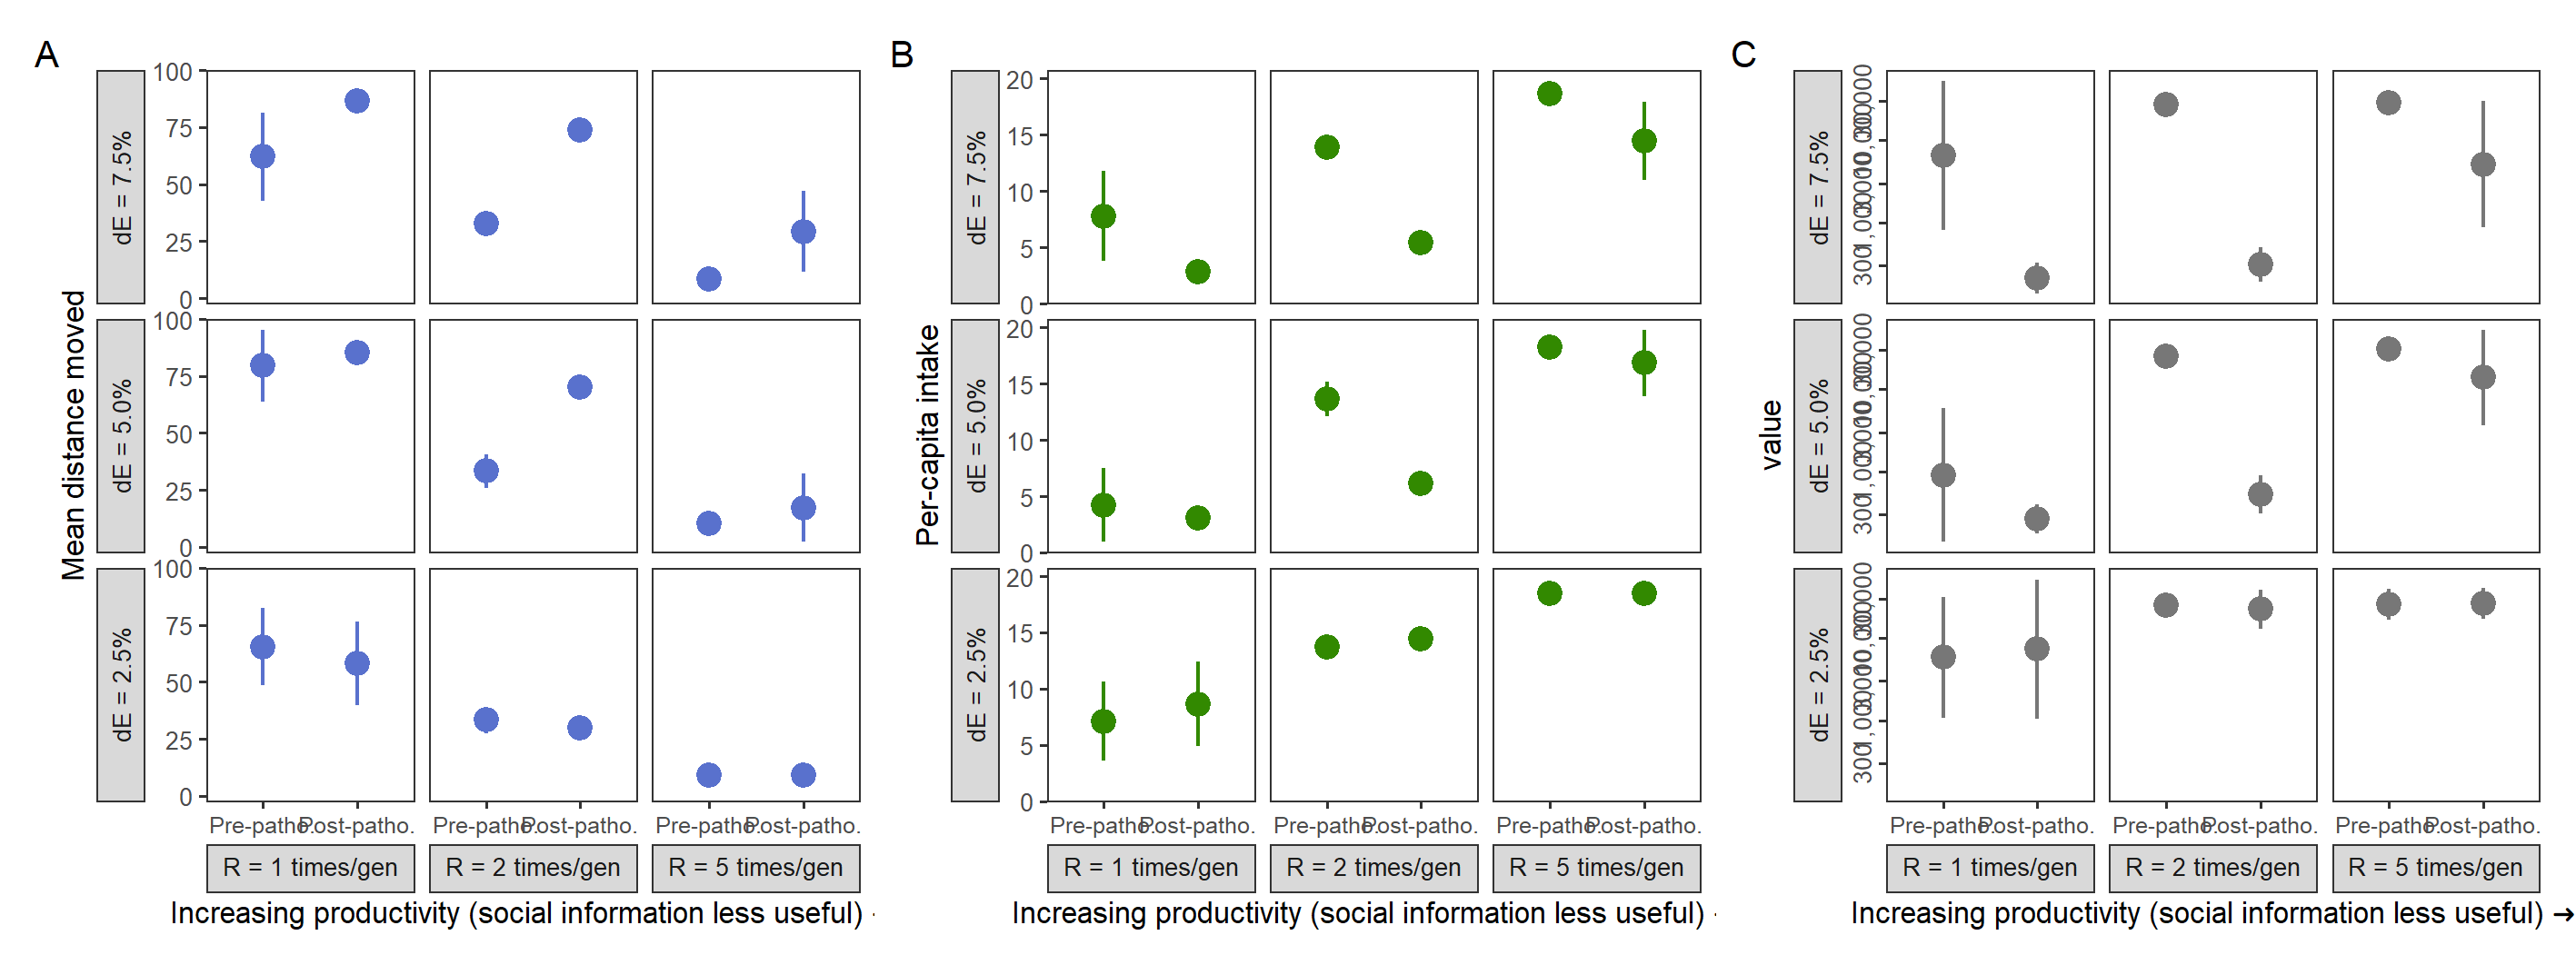
\includegraphics[width=0.95\textwidth]{figures/pathomove/fig_eco_compare_percent.png}
    \caption{
        \textbf{Rapid ecological changes accompany evolutionary shifts in an alternative implementation of disease costs, and are similar to the default implementation.} In the alternative percentage-costs implementation of the infectious pathogen, the outcomes are very similar to those in our default implementation of direct costs. Across most parameter combinations, there is an increase in movement, a reduction in intake, and a reduction in associations with other foragers. Each subplot in each panel shows the mean and standard error of the per-capita values for \textbf{(A)} distance moved, \textbf{(B)} intake, \textbf{(C)} number of associations, or encounters, with other individuals. Means and standard deviations are shown before (G = 3,000) and after (G = 3,500) pathogen introduction; each data point represents 10 replicates of the relevant parameter combination.
    }
\end{figure}

\subsection*{Sporadic Introduction of Infectious Pathogens}

We implemented a variant of our main model, in which the infectious pathogen is introduced only sporadically after the first introduction event (at G = 3,000).
Specifically, we modelled probabilistic introduction of the pathogen in each generation following the initial introduction.
We call the per-generation probability of a novel pathogen introduction event the `spillover rate'.
We ran 10 replicates each of this model variant and examined whether there was a similar evolutionary shift in social movement strategies as seen in our default implementation.
Since it is the main parameter of interest, we ran this model variant for three values of the spillover rate: 0.05, 0.1, and 0.25.
Instead of examining the joint effect of landscape productivity and cost of infection as well, we only examined the effect of infection cost, implementing three different variants with an infection cost \(\delta E\) of 0.1, 0.25, and 0.5.
We kept all other model parameters similar to the default scenario of our main model, and importantly, considered only a landscape productivity \(R\) of 2.
Cross-species novel pathogen introductions are likely to become more common with climate change, and so we chose these spillover rate values to represent different scenarios under altered global regimes of pathogen transfer.
Our model's default implementation may be seen as an extreme case of the models considered here, with a spillover rate of 1.0.

In our model code, the sporadic introduction is implemented by drawing the number of generations until the next pathogen introduction event from a geometric distribution whose probability parameter is given by the spillover rates described above.
Zero values are handled by converting them into ones.
At our lowest spillover rate, up to 100 generations could pass between pathogen introductions, while at our highest rates, there are rarely more than 10 generations between introductions.

The social movement strategies evolved prior to pathogen introduction are identical to those seen in our default implementation, as expected.
However, following pathogen introduction, we found that there was little to change in the population-level mixture of movement strategies in this model variant (see figure).
This is regardless of the probability of a novel pathogen introduction (our so-called `spillover rate'), and the cost of infection by a pathogen.
Across the simulation, the commonest social movement strategy remains `agent tracking', i.e., preferring locations with multiple individuals regardless of their foraging status.
Since there is little to no change in social movement strategies, we did not expect nor find changes in ecological outcomes.

\begin{figure}
    \centering
    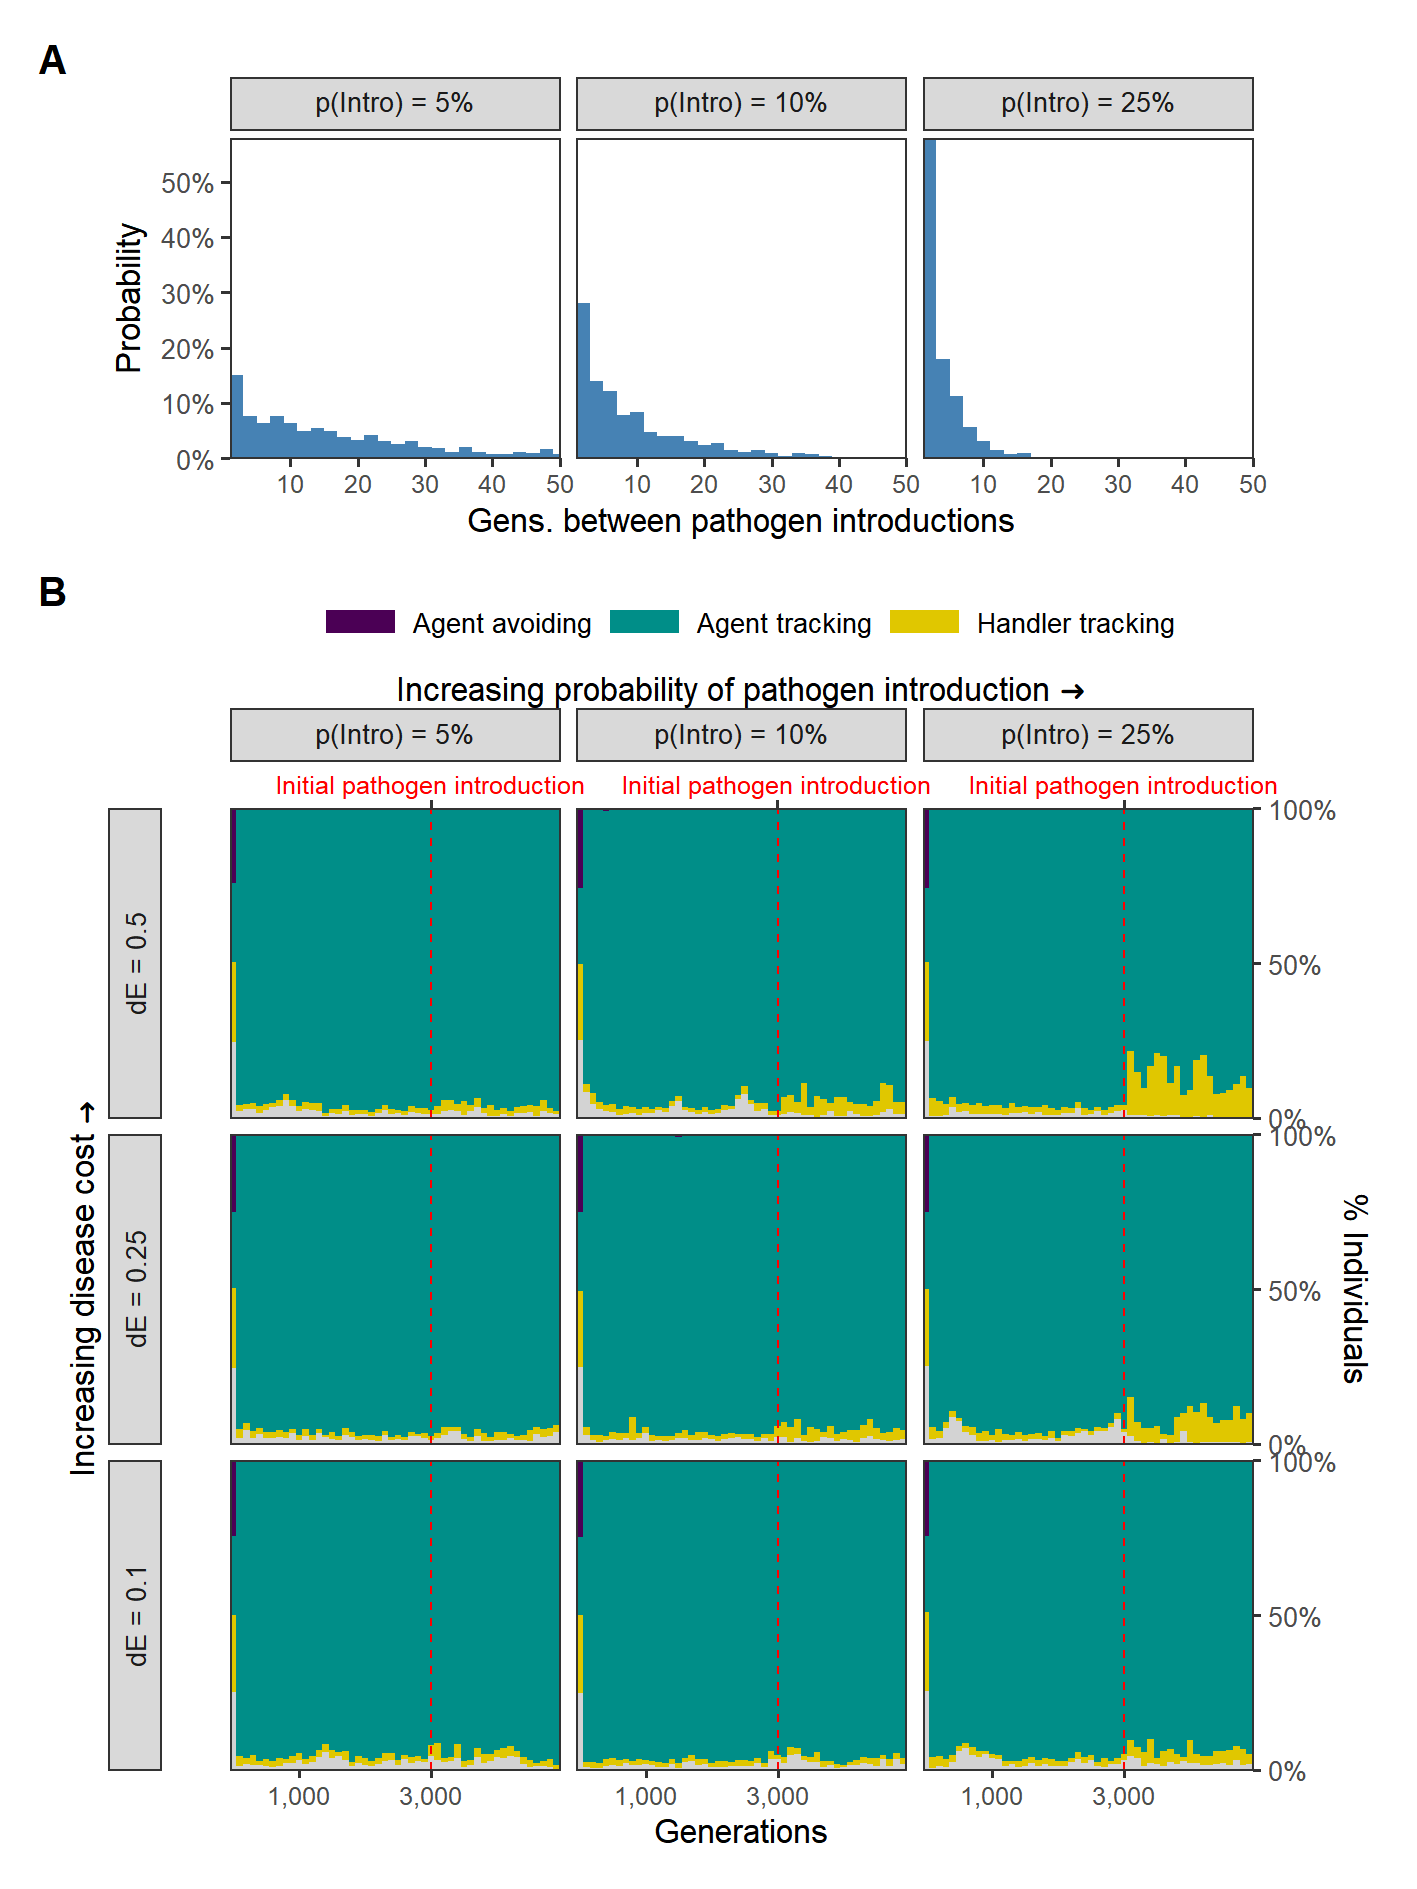
\includegraphics[width=0.7\textwidth]{figures/pathomove/fig_evo_strategy_sporadic.png}
    \caption{\textbf{No evolutionary change in social movement strategies when novel pathogen introduction events are relatively uncommon.} \textbf{(A)} In our alternative implementation of the model, the pathogen is only introduced sporadically after the initial introduction (G = 3,000; red line in panel B). \textbf{(B)} When the introductions are relatively rare and sporadic, there is no shift in the mixture of movement strategies after pathogen introduction. The agent tracking strategy remains common across parameter combinations.}
\end{figure}

{ \begin{center} \barfont{-.-} \end{center} }

\endgroup

